% !TEX program = pdflatex
%!TEX spellcheck
%% For double-blind review submission, w/o CCS and ACM Reference (max submission space)
\documentclass[acmsmall,review,anonymous]{acmart}\settopmatter{printfolios=true,printccs=false,printacmref=false}
%% For double-blind review submission, w/ CCS and ACM Reference
%\documentclass[acmsmall,review,anonymous]{acmart}\settopmatter{printfolios=true}
%% For single-blind review submission, w/o CCS and ACM Reference (max submission space)
%\documentclass[acmsmall,review]{acmart}\settopmatter{printfolios=true,printccs=false,printacmref=false}
%% For single-blind review submission, w/ CCS and ACM Reference
%\documentclass[acmsmall,review]{acmart}\settopmatter{printfolios=true}
%% For final camera-ready submission, w/ required CCS and ACM Reference
%\documentclass[acmsmall]{acmart}\settopmatter{}


%% Journal information
%% Supplied to authors by publisher for camera-ready submission;
%% use defaults for review submission.
\acmJournal{PACMPL}
\acmVolume{1}
\acmNumber{CONF} % CONF = POPL or ICFP or OOPSLA
\acmArticle{1}
\acmYear{2018}
\acmMonth{1}
\acmDOI{} % \acmDOI{10.1145/nnnnnnn.nnnnnnn}
\startPage{1}

%% Copyright information
%% Supplied to authors (based on authors' rights management selection;
%% see authors.acm.org) by publisher for camera-ready submission;
%% use 'none' for review submission.
\setcopyright{none}
%\setcopyright{acmcopyright}
%\setcopyright{acmlicensed}
%\setcopyright{rightsretained}
%\copyrightyear{2018}           %% If different from \acmYear

%% Bibliography style
\bibliographystyle{ACM-Reference-Format}
%% Citation style
%% Note: author/year citations are required for papers published as an
%% issue of PACMPL.
\citestyle{acmauthoryear}   %% For author/year citations


%%%%%%%%%%%%%%%%%%%%%%%%%%%%%%%%%%%%%%%%%%%%%%%%%%%%%%%%%%%%%%%%%%%%%%
%% Note: Authors migrating a paper from PACMPL format to traditional
%% SIGPLAN proceedings format must update the '\documentclass' and
%% topmatter commands above; see 'acmart-sigplanproc-template.tex'.
%%%%%%%%%%%%%%%%%%%%%%%%%%%%%%%%%%%%%%%%%%%%%%%%%%%%%%%%%%%%%%%%%%%%%%


%% Some recommended packages.
\usepackage{booktabs}   %% For formal tables:
                        %% http://ctan.org/pkg/booktabs
\usepackage{subcaption} %% For complex figures with subfigures/subcaptions
                        %% http://ctan.org/pkg/subcaption

\usepackage{algorithm}
\usepackage{tabularx}
\usepackage{algorithmic}
\usepackage{proof}
\usepackage{alltt}
\usepackage{pgf}
\usepackage{tikz}
\usetikzlibrary{arrows,automata}
\usepackage{bcproof}


\renewcommand{\algorithmicrequire}{\textbf{Input:}}

\renewcommand{\algorithmicensure}{\textbf{Output:}}

\newtheorem{Def}{Defination}[section]
\newtheorem{mythm}{Theorem}[section]
\newtheorem{lemma}{Lemma}[section]
\newtheorem{Asm}{Assumption}

\newcommand{\Code}[1]{\texttt{#1}}
\newenvironment{Codes}
  {\begin{alltt}\leftskip=1.5em} % \small
  {\end{alltt}}

\newcommand{\OneStep}{{\rule{0pt}{1.2\baselineskip}{\ensuremath\longrightarrow}}}
\newcommand{\DeStep}{{\rule{0pt}{1.2\baselineskip}{\ensuremath\dashrightarrow}}}

\newcommand\m[1]{\mbox{\tt #1}}
\newcommand\key[1]{\mbox{\rm \bf #1}}
\newcommand\drule[2]{#1 ~\rightarrow_d~ #2}
\newcommand\redc[2]{#1 ~\rightarrow_c~#2}
\newcommand\rede[2]{#1 ~\rightarrow_e~#2}
\newcommand\redm[2]{#1 ~\rightarrow_m~#2}
\newcommand\note[1]{\mbox{{\small #1}}}
\newcommand\ignore[1]{}

\def\coreId{\m{cId}}
\def\surfId{\m{sId}}
\def\headId{\m{hId}}

\def\true{\#t}
\def\false{\#f}

% some macros for editing/commenting the paper

\def\modify#1#2#3{{\small\underline{\sf{#1}}:} {\color{red}{\small #2}}
{{\color{red}\mbox{$\Rightarrow$}}} {\color{blue}{#3}}}

\newcommand{\hmodify}[2]{\modify{Hu}{#1}{#2}}
\newcommand\mymargin[1]{\marginpar{{\flushleft\textsc\footnotesize {#1}}}}
\newcommand\hmargin[1]{\mymargin{Hu:\;#1}}

\newcommand{\hmodifyok}[2]{#2}

\newcommand{\mycomment}[2]{{\small\color{magenta}\underline{\sf{#1}}:} {\color{magenta}{\small #2}}}
\newcommand{\hcomment}[1]{\mycomment{Hu}{#1}}
\newcommand{\todo}[1]{\mycomment{Todo}{#1}}

\begin{document}

%% Title information
\title%[Short Title]
{Lifting Resugaring by Lazy Desugaring}
%{A lightweight resugaring approach based on reduction semantics}
%% [Short Title] is optional;
                                        %% when present, will be used in
                                        %% header instead of Full Title.
%\titlenote{with title note}             %% \titlenote is optional;
                                        %% can be repeated if necessary;
                                        %% contents suppressed with 'anonymous'
%\subtitle{Subtitle}                     %% \subtitle is optional
%\subtitlenote{with subtitle note}       %% \subtitlenote is optional;
                                        %% can be repeated if necessary;
                                        %% contents suppressed with 'anonymous'


%% Author information
%% Contents and number of authors suppressed with 'anonymous'.
%% Each author should be introduced by \author, followed by
%% \authornote (optional), \orcid (optional), \affiliation, and
%% \email.
%% An author may have multiple affiliations and/or emails; repeat the
%% appropriate command.
%% Many elements are not rendered, but should be provided for metadata
%% extraction tools.

%% Author with single affiliation.
\author{First1 Last1}
\authornote{with author1 note}          %% \authornote is optional;
                                        %% can be repeated if necessary
\orcid{nnnn-nnnn-nnnn-nnnn}             %% \orcid is optional
\affiliation{
  \position{Position1}
  \department{Department1}              %% \department is recommended
  \institution{Institution1}            %% \institution is required
  \streetaddress{Street1 Address1}
  \city{City1}
  \state{State1}
  \postcode{Post-Code1}
  \country{Country1}                    %% \country is recommended
}
\email{first1.last1@inst1.edu}          %% \email is recommended

%% Author with two affiliations and emails.
\author{First2 Last2}
\authornote{with author2 note}          %% \authornote is optional;
                                        %% can be repeated if necessary
\orcid{nnnn-nnnn-nnnn-nnnn}             %% \orcid is optional
\affiliation{
  \position{Position2a}
  \department{Department2a}             %% \department is recommended
  \institution{Institution2a}           %% \institution is required
  \streetaddress{Street2a Address2a}
  \city{City2a}
  \state{State2a}
  \postcode{Post-Code2a}
  \country{Country2a}                   %% \country is recommended
}
\email{first2.last2@inst2a.com}         %% \email is recommended
\affiliation{
  \position{Position2b}
  \department{Department2b}             %% \department is recommended
  \institution{Institution2b}           %% \institution is required
  \streetaddress{Street3b Address2b}
  \city{City2b}
  \state{State2b}
  \postcode{Post-Code2b}
  \country{Country2b}                   %% \country is recommended
}
\email{first2.last2@inst2b.org}         %% \email is recommended


%% Abstract
%% Note: \begin{abstract}...\end{abstract} environment must come
%% before \maketitle command
\begin{abstract}


Syntactic sugar, first coined by Peter J. Landin in 1964, has proved to be very useful for defining domain-specific languages and extending languages.
  Unfortunately, when syntactic sugar is eliminated by transformation, it obscures the relationship between the user’s source program and the transformed program.
Resugaring is a powerful technique to resolve this problem, which automatically converts the evaluation sequences of desugared expression in the core language into representative sugar's syntax in the surface language. However, the traditional approach
relies on reverse application of desugaring rules to desugared core expression whenever possible. When a desugaring rule is complex and a desugared expression is large, such reverse desugaring becomes very complex  and costive.

In this paper, we propose a novel approach to resugaring by lazy desugaring, where reverse application of desugaring rules is unnecessary. We recognize a sufficient and necessary condition for a syntactic sugar to be desugared, and propose a reduction strategy, based on evaluator of the core languages and the desugaring rules, which is sufficient to produce all necessary resugared terms on the surface language. We show that this approach can be made more efficient by automatic derivation of evaluation rules for syntactic sugars.
We have implemented a system based on this new approach. Compared to the traditional approach, the new approach is not only more efficient, but also more powerful in that it cannot only deal with all cases (such as hygienic and simple recursive sugars) published so far, but can do more allowing more flexible recursive sugars.

\end{abstract}


%% 2012 ACM Computing Classification System (CSS) concepts
%% Generate at 'http://dl.acm.org/ccs/ccs.cfm'.
\begin{CCSXML}
<ccs2012>
<concept>
<concept_id>10011007.10011006.10011008</concept_id>
<concept_desc>Software and its engineering~General programming languages</concept_desc>
<concept_significance>500</concept_significance>
</concept>
<concept>
<concept_id>10003456.10003457.10003521.10003525</concept_id>
<concept_desc>Social and professional topics~History of programming languages</concept_desc>
<concept_significance>300</concept_significance>
</concept>
</ccs2012>
\end{CCSXML}

\ccsdesc[500]{Software and its engineering~General programming languages}
\ccsdesc[300]{Social and professional topics~History of programming languages}
%% End of generated code


%% Keywords
%% comma separated list
\keywords{Resugaring, Syntactic Sugar, Interpreter, Domain-specific language, Reduction Semantics}  %% \keywords are mandatory in final camera-ready submission


%% \maketitle
%% Note: \maketitle command must come after title commands, author
%% commands, abstract environment, Computing Classification System
%% environment and commands, and keywords command.
\maketitle

%!TEX root = ./main.tex
\section{Introduction}

%What is the research background and and what motivate you to do this research?

%What is the research issue and how the issue has been addressed so far?

%What is the remained research problem and how challenge it is?

%What is your key idea (insight) of your solution to be discussed in this paper?

%What are the three main technical contributions of this paper?

%The rest of the paper is organized as follows. ...

Domain-specific language\cite{dsl} is becoming useful for people's daily tasks. For example, the IFTTT app and IOS's shortcuts designed DSLs describing some tasks to make our lives more convenient. So the users of DSL are no longer limited to programmers, but people from all walks of life.(to be completed)

Syntactic sugar\cite{syntacticsugar}, as a simple ways design DSL, has a obvious problem. DSL based on syntactic sugars contains many components of its host language. Then its interpretation will be outside the DSL itself. The evaluation sequences of syntactic sugar expression will contain many terms of the host language, which may confuse the users of DSL.

There is an existing work---resugaring\cite{resugaring}\cite{hygienic}, which aimed to solve the problem upon. It lifts the evaluation sequences of desugared expression to sugar's syntax. The evaluation sequences shown by resugaring will not contain components of host language. But we found the resugaring method using match and substitution is kind of redundant. The biggest deficiency of existing resugaring method is that the syntactic sugars in an expression have to fully desugar before evaluation. This limits the processing ability of the method. Moreover, it limits the complexity of getting the resugaring sequences. If we need to resugar a very huge expression, the match and substitution processes will cost so much. Also, processing of hygienic macros is complex due to the extra data structure.

In this paper, We propose a lightweight approach to get resugaring sequences based on syntactic sugars. The key idea of our approach is---syntactic sugar expression only desugars at the point that it have to desugar. We guess that we don't have to desugar the whole expression at the initial time of evaluation under the premise of keeping the properties of expression. 

Initially, our work focused on improving current resugaring method. After finishing that, we found our lightweight resugaring approach could process some syntactic sugars' feature that current approach cannot do. Finally, we implement our algorithm using PLT Redex\cite{SEwPR} and test our approach on some applications. The result shows that our approach does handle more features of syntactic sugar.

In the rest of this paper, we present the technical details of our approach together with the proof of correctness. In details, the rest of our paper is organized as follow:

\begin{itemize}
\item An overview of our approach with some background knowledge.[sec \ref{sec2}]
\item The algorithm defination and proof of correctness.[sec \ref{sec3}]
\item The implementation of our lightweight resugaring algorithm using PLT Redex.[sec \ref{sec4}]
\item sth else?[sec \ref{sec5}]
\item Evaluation of our lightweight resugaring approach.[sec \ref{sec6}]
\end{itemize}

%!TEX root = ./main.tex
\section{Overview}
\label{sec2}


In this section, we give a brief overview of our approach. To be concrete, we will consider the following simple core language, defining boolean expressions using the \m{if} construct:
\[
\begin{array}{lllll}
e &::=& \m{CoreExp}\\
\m{CoreExp} &::=& \Code{(if~$e$~$e$~$e$)} &\note{// if construct}\\
& |& \true  & \note{// true value}\\
& |& \false & \note{// false value}
\end{array}
\]
The semantics of the language is simple, consisting of the following context rule to specify the computational order:
\[
\begin{array}{lcl}
C &:=& \Code{(if C $e$ $e$)}\\
&|&[\bigcdot] \qquad \note{//evaluation context's hole}\\
\end{array}
\]
and two reduction rules (the letter c means core):
\[
\centering
 \redc{(\m{if}~\true~e_1~e_2)}{e_1}  \qquad \redc{(\m{if}~\false~e_1~e_2)}{e_2}
\]
Assume that our surface language is defined by two syntactic sugars defined by:
%---\emph{and} sugar and \emph{or} sugar on the core language.
\[
\begin{array}{c}
\drule{(\m{And}~e_1~e_2)}{(\m{if}~e_1~e_2~\false)}\\
\drule{(\m{Or}~e_1~e_2)}{(\m{if}~e_1~\true~e_2)}
\end{array}
\]
Now let us demonstrate how to execute \Code{(And (Or \true~\false) (And \false ~\true))}, and get the following resugaring sequence by our approach.
{\small
\begin{Codes}
    (And (Or \true \false) (And \false \true))
\OneStep{ (And \true (And \false \true))}
\OneStep{ (And \false \true)}
\OneStep{ #f}
\end{Codes}
}

Our new resugaring approach eliminates costive "reverse desugaring" by "lazy desugaring", where a syntactic sugar will be expanded only when it is necessary. It consists of following three steps.

{\em Step 1: Calculating Context Rules for Sugars.}
While giving the evaluation rules of the core language, we can derive the following context rules of the surface language.
\[
\begin{array}{lcl}
C &:=& (\m{And}~C~e)\\
&|& (\m{Or}~C~e)\\
&|&[\bigcdot]\\
\end{array}
\]
From the context rules of \m{if}, we can find that the condition ($e_1$) is always evaluated first. Therefore, for expression \Code{(And $e_1$ $e_2$)} defined by syntactic sugar, $e_1$ is also evaluated first, which is the context rule of \m{And}. Similarly, we can calculate the context rule of \m{Or}.

{\em Step 2: Deriving Reduction Rules for the Mixed Language.}
We mix the surface language with the core language as in Fig. \ref{fig:mixexample}, where \m{CommonExp} means the expressions used in both the surface language and the core language both, and derive $\to_m$, a one-step reduction in our mixed language, from the the reduction rules of fhe core language and the given desugaring rules. By using $\to_m$, we can get the following evaluation sequence in the mixed language for
the program \Code{(And (Or \true~\false) (And \false~\true))}

{\footnotesize
\begin{Codes}
    (And (Or \true \false) (And \false \true))
\OneStep{ (And (if \true \true \false) (And \false \true))}
\OneStep{ (And \true (And \false \true))}
\OneStep{ (if \true (And \false \true) \false)}
\OneStep{ (And \false \true)}
\OneStep{ (if \false \true \false)}
\OneStep{ \false}
\end{Codes}
}


\begin{figure}[t]
\centering
\begin{subfigure}{\linewidth}{\footnotesize
    \begin{flushleft}
        \[
        \begin{array}{lll}
        e &::=& \m{CoreExp} \\
        &|&\m{SurfExp}\\
        &|&\m{CommonExp}\\
        \m{CoreExp} &::=& \Code{(if~$e$~$e$~$e$)}\\
        \m{SurfExp} &::=& \Code{(And~$e$~$e$)}\\
        &|&\Code{(Or~$e$~$e$)}\\
        \m{CommonExp} &::=& \true\\
        &|& \false\\
        \end{array}
        \]
    \end{flushleft}
    \caption{Syntax}
    \label{fig:mixsyntax}
}
\end{subfigure}
\begin{subfigure}{\linewidth}{\footnotesize
    \begin{flushleft}
        \[\footnotesize
        \begin{array}{lcl}
        C &:=& (\m{if}~C~$e$~$e$)\\
        &|& (\m{And}~C~$e$)\\
        &|& (\m{Or}~C~$e$)\\
        &|&[\bigcdot]\\
        \end{array}
        \]
        \end{flushleft}
    \caption{Context Rules}
    \label{fig:mixcontext}
}
\end{subfigure}

\begin{subfigure}{\linewidth}{\footnotesize
    \begin{flushleft}
        \[
        \begin{array}{c}
        \redm{(\m{And}~e_1~e_2)}{(\m{if}~e_1~e_2~\false)}\\
        \redm{(\m{Or}~e_1~e_2)}{(\m{if}~e_1~\true~e_2)}\\
        \redm{(\m{if}~\true~e_1~e_2)}{e_1}\\
        \redm{(\m{if}~\false~e_1~e_2)}{e_2}
        \end{array}
        \]
    \end{flushleft}
    \caption{Reduction Rules}
    \label{fig:mixreduction}
}
\end{subfigure}

\caption{Mixed Language Example}
\label{fig:mixexample}
\end{figure}


{\em Step 3: Removing Unnecessary Expressions.}
We can just keep the intermediate sequences without \m{Coreexp} in any sub-expressions to get the resugaring sequence above.

%Note that the context rules should restrict the computational order of a sugar expression's sub-expressions, thus we should let the context rules be correct---reflecting what should be executed in the desugared expression.
Note that as the goal of resugaring is to present the evaluation of sugar programs, we are given a way to clearly specify which expression should be outputted. For the example in this section, of course, the sugar \m{And} and \m{Or} should be outputted, and also the boolean values should be. So we set boolean values as \m{CommonExp} in Fig. \ref{fig:mixsyntax}, so that they can be displayed though they are in the core language. By clearly separating what should be displayed, we can always get the resugaring evaluation sequences we need (this is slightly different from the existing approach's setting, as we will discuss in Section \ref{mark:correctness}.)

%!TEX root = ./main.tex

\section{Resugaring by Lazy Desugaring}
\label{sec3}

In this section, we present our new approach to resugaring. Different from the traditional approach that clearly separates the surface and the core languages, we combine them together as one mixed language, allowing users to freely use the language constructs in both languages. We will show that any expression in the mixed language can be evaluated in such a smart way that a sequence of all expressions that are necessarily to be resugared by the traditional approach can be correctly produced.

\subsection{Mixed Language for Resugaring}

\begin{figure}[t]
	\[
	\begin{array}{lllll}
	 &\m{CoreExp} &::=& x  & \note{variable}\\
	       &&~|~& c  & \note{constant}\\
				 &&~|~& (\m{CoreHead}~\m{CoreExp}_1~\ldots~\m{CoreExp}_n) & \note{constructor}\\
	\\
	 &\m{SurfExp} &::=& x  & \note{variable}\\
	       &&~|~& c  & \note{constant}\\
				 &&~|~& (\m{CoreHead}~\m{SurfExp}_1~\ldots~\m{SurfExp}_n) & \note{selected core constructor}\\
					 &&~|~& (\m{SurfHead}~\m{SurfExp}_1~\ldots~\m{SurfExp}_n) & \note{sugar expression}\\
	\end{array}
	\]
	\caption{Core and Surface Expressions}
	\label{fig:expression}
\end{figure}

We will define a mixed language for a given core language and a surface language defined over the core language. An expression in this language will be reduced step by step by the reduction rules for the core language and the desugaring rules for defining the syntactic sugars in the surface language.

\subsubsection{Core Language}

For our host language, we consider its evaluator as a blackbox \todo{need to be corrected.} but with two natural assumptions. First, there is a deterministic stepper in the evaluator which, given an expression in the host language, can deterministically reduce the expression to a new expression. Second, the evaluation of any sub-expression has no side-effect on other parts of the whole expression.

An expression of the core language is defined in Figure \ref{fig:expression}. It is a variable, a constant, or a (language) constructor expression. Here, $\m{CoreHead}$ stands for a language constructor such as $\m{if}$ and $\m{let}$. To be concrete, we will use the core language defined in Figure \ref{fig:core} to demonstrate our approach.

\begin{figure}[t]
\begin{center}
\begin{tabularx}{.9\textwidth}%
{|>{\setlength{\hsize}{.4\hsize}\centering\arraybackslash}X  |>{\setlength{\hsize}{1.6\hsize}\centering\arraybackslash}X|}
%{|*{2}{>{\centering\arraybackslash}X|}}
\hline
Syntax & Reduction rules \\ \hline
(if e e e) &\qquad\qquad\qquad(if \#t e2 e3) $\rightarrow$ e2 \newline ~(if \#f e2 e3) $\rightarrow$ e3\\ \hline
(($\lambda$ (x ...) e) e ...) & (($\lambda$ (x0 x1 ...) e) v0 v1 ...) $\rightarrow$ (let ((x0 v0) (($\lambda$ (x1 ...) e) v1 ...))\\ \hline
(($\lambda_N$ (x ...) e) e ...) & (($\lambda_N$ (x0 x1 ...) e) e0 e1 ...) $\rightarrow$ (let ((x0 e0) (($\lambda_N$ (x1 ...) e) e1 ...))\\ \hline
(let ((x e) ...) e) & (let ((x0 e0) (x1 e1) ...) e) $\rightarrow$ (let ((x1 e1) ...) (subst x0 e0 e))\newline (let () e)  $\rightarrow$ e (where subst is a meta function)\\ \hline
(first e) & (first (list v1 v2 ...)) $\rightarrow$ v1\\ \hline
(rest e) & (rest (list v1 v2 ...)) $\rightarrow$ (list v2 ...)\\ \hline
(empty e) & \qquad\qquad\qquad(empty (list)) $\rightarrow$ \#t \newline (empty (list v1 ...)) $\rightarrow$ \#f\\ \hline
(cons e e) & (cons v1 (list v2 ...)) $\rightarrow$ (list v1 v2 ...)\\ \hline
(op e e) \newline op=+-*/><== & (op v1 v2) $\rightarrow$ arithmetic result\\ \hline
\end{tabularx}
\end{center}
\caption{An Core Language Example}
\label{fig:core}
\end{figure}


%For simplicity, we use the prefix notation. For instance, we write $\m{if-then-else}~e_1~e_2~e_3$, which would be more readable if we write $\m{if}~e_1~\m{then}~e_2~\m{else}~e_3$. In this paper, we may write both if it is clear from the context.

\subsubsection{Surface Language}

Our surface language is defined by a set of syntactic sugars, together with some language constructs in the core language. So an expression of the surface language is some core constructor expressions with sugar expressions, as defined in Figure \ref{fig:expression}.

A syntactic sugar is defined by a desugaring rule in the following form:
\[
\drule{(\m{SurfHead}~x_1~x_2~\ldots~x_n)}{\m{SurfExp}}
\]
where its LHS is a simple pattern (unnested) and its RHS is a surface expression. For instance, we may define syntactic sugar \m{And} by
\[
\drule{(\m{And}~x~y)}{\m{if}~x~y~\false}.
\]
Note that if the pattern is nested, we can introduce a new syntactic sugar to flatten it.
One may wonder why not restricting the RHS to be a core expression $\m{CoreExp}$, which sounds more natural. We use $\m{surfExp}$ to be able to allow definition of recursive syntactic sugars, as seen in the following example.
\[
\begin{array}{l}
\drule{(\m{Odd}~x)}{\m{if}~(>~x~0)~(\m{Even}~(−~x~1))~\false)}\\
\drule{(\m{Odd}~x)}{\m{if}~(>~x~0)~(\m{Odd}~(−~x~1))~\true)}
\end{array}
\]

We assume that all desugaring rules are not overlapped in the sense that for a syntactic sugar expression, only one desugaring rule is applicable.

\ignore{
\subsubsection{Grammatical restrictions}
Firstly, the whole language should be restricted to tree-structured disjoint expression.

\begin{Def}[disjoint]
For every sub-expression in a expression, its reduction rule is decided by itself.
\end{Def}

This restriction limits the scope of language. Every sub-expression must have no side effect. We will discuss more on side effect in ...

\begin{Def}[tree-structured]
The grammar of the whole language is defined as follow.
\[
\begin{array}{rcl}
\mbox{Exp} &::=& (\mbox{Headid}~\mbox{Exp}*)\\
&|& \mbox{Value}\\
&|& \mbox{Variable}
\end{array}
\]
\end{Def}

The grammatical restrictions give our language a similiar property as church-rosser theorem for lambda calculus.

todo:church-rosser?

\subsubsection{Context restrictions}
For expressions in CoreLang, the context rules should restrict it to have only one reduction path. The context rules can limit the order of evaluation. This restriction is normal, because a program in general-purposed language should have only one execution path.\label{mark:ctx}

For expressions in SurfLang, context rules should allow every sub-expressions reduced. It's the same as full-$\beta$ reduction.

\subsubsection{Restriction of syntactic sugar}
The form of syntactic sugar is as follow.

\fbox{
$(\mbox{Surfid}\;e_{1}\;e_{2}\;\ldots)$ ~→~ $(\mbox{Headid}\; \ldots)$
}

An counter example of this restriction is $(\mbox{Surfid}\;\ldots\;(e1\;e2)\ldots))$ in LHS. It's for simpler algorithm form, and the expression ability of syntactic sugar will not be changed.

\begin{Def}[Unambiguous]
For every syntactic sugar expressions, it can only desugar to one expression in CoreLang.
\end{Def}

}

\subsubsection{Mixed Language}

\begin{figure}[t]
\begin{centering}
	\framebox[36em][c]{
		\parbox[t]{33em}{
			\[
			\begin{array}{lcl}
			\m{Exp} &::=& \m{DisplayableExp}\\
			&|& \m{UndisplayableExp}\\
\\
			\m{DisplayableExp} &::=& \m{SurfExp}\\
			&|& \m{CommonExp}
\\
			\m{UndisplayableExp} &::=& \m{CoreExp}\\
			&|& \m{OtherSurfExp}\\
			&|& \m{OtherCommonExp}\\
\\
			\m{CoreExp} &::=& (\m{CoreHead}~\m{Exp}*)\\
\\
			\m{SurfExp} &::=& (\m{SurfHead}~\m{DisplayableExp}*)\\
\\
			\m{CommonExp} &::=& (\m{CommonHead}~\m{DisplayableExp}*)\\
			&|& c \qquad \note{// constant value}\\
			&|& x \qquad \note{// variable} \\
\\
			\m{OtherSurfExp} &::=& (\m{SurfHead}~\m{Exp}*~\m{UndisplayableExp}~\m{Exp}*)\\
\\
			\m{OtherCommonExp} &::=& (\m{CommonHead}~\m{Exp}*~\m{UndisplayableExp}~\m{Exp}*)
			\end{array}
			\]
		}
	}
\end{centering}
\caption{Our Mixed Language}
\label{fig:mix}
\end{figure}

Our mixed language for resugaring combines the surface language and the core language.
%
The difference between our core language (CoreLang) and our surface language (SurfLang) is identified by $\m{HeadId}$. But there are some terms in the core language should be displayed during evaluation, or we need some terms to help us getting better resugaring sequences. So we defined \m{CommonExp}, which origin from CoreLang, but can be displayed in resugaring sequences. The \m{CoreExp} terms are terms with undisplayable CoreLang's \m{Headid}. The \m{SurfExp} terms are terms with SurfLang's \m{Headid} and all sub-expressions are displayable. The \m{CommonExp} terms are terms with displayable CoreLang's Headid, together with displayable sub-expressions. There exists some other expression during our resugaring process, which have \m{Headid} which can be displayed, but one or more subexpressions cannot. They are \m{UndisplayableExp}.
\todo{Do we need \m{HeadId}?}

Take some terms in the core language in Figure \ref{fig:core} as examples.
We may assume \m{if}, \m{let}, \m{$\lambda _{N}$}, \m{empty}, \m{first}, \m{rest} as \m{CoreExp}'s \m{Headid}, \m{op}, \m{$\lambda$}, \m{cons} as \m{CommonExp}'s \m{Headid}. Then we could show some useful intermediate steps.


\subsection{Resugaring Algorithm}

Our resugaring algorithm works on our mixed language, based on the reduction rules of the core language and the desugaring rules for defining the surface language. Let $\redc{}{}$ denote a one-step reduction of the core language, and $\drule{}{}$ a one-step desugaring by a desuaring rule. We define $\redm{}{}$, a one-step reduction of our mixed language, as follows.

\infrule[CoreRed]
{\redc{(\m{CoreHead}~e_1~\ldots~e_n)}{e'}}
{\redm{(\m{CoreHead}~e_1~\ldots~e_n)}{e'}}

\infrule[SurfaceRed]
{\drule{(\m{SurfHead}~x_1~\ldots~x_i~\ldots~x_n)}{e}\\
 \redm{e[e_1/x,\ldots,e_i/x_i,\ldots,e_n/x_n]}{e[e_1/x,\ldots,e_i'/x_i,\ldots,e_n/x_n]}
}
{\redm{(\m{SurfHead}~e_1~\ldots~e_i~\ldots~e_n)}{(\m{SurfHead}~e_1~\ldots~e_i'~\ldots~e_n)}}


Our resugaring algorithm is based on a core algorithm f. For every expression during resugaring process, it may have one or more reduction rules. The core algorithm f chooses the one that satisfies three properties of resugaring, then applies it on the given expression. The core algorithm f is defined as \ref{alg:f}.
\begin{algorithm}
	\caption{Core-algorithm f}
	\label{alg:f}     % 给算法一个标签,以便其它地方引用该算法
	\begin{algorithmic}[1]       % 数字 "1" 表示为算法显示行号的时候,每几行显示一个行号,如:"1" 表示每行都显示行号,"2" 表示每两行显示一个行号,也是为了方便其它地方的引用
		\REQUIRE ~~\\      % 算法的输入参数说明部分
		Any expression $Exp$=$(Headid~Subexp_{1}~\ldots~Subexp_{\ldots})$ which satisfies Language setting
		\ENSURE ~~\\     % 算法的输出说明
		$Exp'$ reduced from $Exp$, s.t. the reduction satisfies three properties of resugaring
		\STATE     Let $ListofExp'$ = $\{Exp'_{1}\;,Exp'_{2}~\ldots\}$
		\IF {$Exp$ is Coreexp or  Commonexp or OtherCommonexp}
		\IF {Lengthof($ListofExp'$)==0}
		\RETURN null; \hfill Case1
		\ELSIF {Lengthof($ListofExp'$)==1}
		\RETURN first($ListofExp'$); \hfill Case2
		\ELSE
		\RETURN $Exp'_{i}$ = $(Headid~Subexp_{1}~\ldots~Subexp'_{i}~\ldots)$; //where i is the index of subexp which have to be reduced. \hfill Case3
		\ENDIF
		\ELSE
		\IF {$Exp$ have to be desugared}
		\RETURN desugarsurf($Exp$); \hfill Case4
		\ELSE
		\STATE Let $DesugarExp$ = desugarsurf(Exp)
		\IF {$Subexp_{i}$ is reduced to $Subexp'_{i}$ during $f(DesugarExp)$}
		\RETURN $Exp'_{i}$ = $(Headid~Subexp_{1}~\ldots~Subexp'_{i}~\ldots)$; \hfill Case5
		\ELSE
		\RETURN $DesugarExp$; \hfill Case6
		\ENDIF
		\ENDIF
		\ENDIF

	\end{algorithmic}
\end{algorithm}

We briefly describe the core algorithm f in words.

For Exp in language defined as last section, try all reduction rules in the language, get a list of possible expressions ListofExp'=\{$Exp'_{1}$,$Exp'_{2}$,$\ldots$\}.

Line 2-9 deal with the case when Exp has a CoreLang's Headid. When Exp is value or variable (line 3-4), ListofExp' won't have any element (not reducible). When Exp is of Coreexp or Commonexp (line 5-6), due to the context restriction of CoreLang, only one reduction rule can be applied. When Exp is OtherCommonexp (line 7-8), due to the context restriction of CoreLang, only one sub-expression can be reduced, then just apply core algorithm recursively on the sub-expression.

Line 10-21 deal with the case then Exp has a SurfLang's Headid. When Exp only has one reduction rule (line 11-12), the syntactic sugar has to desugar. If not, we should expand outermost sugar and find the sub-expression which should be reduced (line 14-16), or the sugar has to desugar (line 17-18), because it will never be resugared. The steps in line 14 to 16 are the critical part of our algorithm (call {\bfseries one-step try}\label{mark:onesteptry}).


Then, our lightweight-resugaring algorithm is defined as \ref{alg:lwresugar}.

\begin{algorithm}
	\caption{Lightweight-resugaring}
	\label{alg:lwresugar}     % 给算法一个标签,以便其它地方引用该算法
	\begin{algorithmic}[1]       % 数字 "1" 表示为算法显示行号的时候,每几行显示一个行号,如:"1" 表示每行都显示行号,"2" 表示每两行显示一个行号,也是为了方便其它地方的引用
		\REQUIRE ~~\\      % 算法的输入参数说明部分
		Surfexp $Exp$
		\ENSURE ~~\\     % 算法的输出说明
		$Exp$'s evaluation sequences within DSL
		\WHILE {$tmpExp$ = f($Exp$)}
		\IF {$tmpExp$ is empty}
		\RETURN
		\ELSIF {$tmpExp$ is Surfexp or Commonexp}
		\PRINT $tmpExp$;
		\STATE Lightweight-resugaring($tmpExp$);
		\ELSE
		\STATE Lightweight-resugaring($tmpExp$);
		\ENDIF
		\ENDWHILE

	\end{algorithmic}
\end{algorithm}

The whole process of the lightweight resugaring executes core algorithm f, and output sequences which is of Surfexp or Commonexp.

\subsection{Proof of correctness}

First of all, because the difference between our lightweight resugaring algorithm and the existing one is that we only desugar the syntactic sugar when needed, and in the existing approach, all syntactic sugar desugars firstly and then executes on CoreLang.

Second, to prove convenience, define some terms.

$Exp~=~(Headid\;Subexp_{1}\;Subexp_{\ldots} \ldots)$ is any reducible expression in our language.

If we use the reduction rule that desugar Exp's outermost syntactic sugar, then the reduction process is called {\bfseries Outer Reduction}.

If the reduction rule we use reduce $Subexp_{i}$, where $Subexp_{i}$ is $(Headid_{i}~Subexp_{i1}~Subexp_{i\ldots} \ldots)$
\begin{itemize}
	\item If the reduction process is Outer Reduction of $Subexp_{i}$ = $(Headid_{i}~Subexp_{i1}~Subexp_{i\ldots} \ldots)$, then it is called {\bfseries Surface Reduction}.
	\item If the reduction process reduces $Subexp_{ij}$, then it is called {\bfseries Inner Reduction}.
\end{itemize}

{\bfseries Example:}

$(\mbox{if}\; \#t\; Exp_{1}\; Exp_{2})$ → $Exp1$ \hfill Outer Reduction

$(\mbox{if}\; (\mbox{And}\; \#t\; \#f)\; Exp_{1}\; Exp_{2})$ → $(\mbox{if}\; (\mbox{if}\; \#t\; \#f\; \#f)\; Exp_{1}\; Exp_{2})$ \hfill Surface Reduction

$(\mbox{if}\; (\mbox{And}\; (\mbox{And}\; \#t\; \#t)\; \#t)\; \#f)\; Exp_{1}\; Exp_{2})$ → $(\mbox{if}\; (\mbox{And}\; \#t\; \#t)\; Exp_{1}\; Exp_{2})$ \hfill Inner Reduction

\begin{Def}[Upper and lower expression]
For $Exp$=$(Headid\;Subexp_{1}\;Subexp_{\ldots} \ldots)$, $Exp$ is called {\bfseries upper expression}$,Subexp_{i}$is called {\bfseries lower expression}.
\end{Def}

We only need to prove that all the 6 cases of core algorithm f won't effect its properties. Case 1 and case 3 won't effect any properties, because it does what CoreLang should do.

\begin{proof}[Proof of Emulation]
\hfill\\
For case 4 and 6, desugaring won't change Emulation property, because desugaring and resugaring are interconvertible.

For case 2 and 5, our core algorithm reduces the sub-expression which should be reduced. So if applying core algorithm f on the subexpression satisfies emulation property, then this two cases satisfy. A recursive proof it is.
todo:case5
\end{proof}

\begin{proof}[Proof of Abstraction]
\hfill\\
It's true, because we only display the sequence which satisfies abstraction property.
\end{proof}

\begin{lemma}
If no syntactic sugar desugared before it has to, then coverage property is satisfied.
\end{lemma}

\begin{proof}[Proof of Lemma]
Assume that no syntactic sugar not necessarily expanded desugars too early, existing an expression in CoreLang

$Exp$ = $(Headid\;Subexp_{1}\;Subexp_{\ldots} \ldots)$ which can be resugared to

$ResugarExp'$ = $(Surfid\;Subexp'_{1}\;Subexp'_{\ldots}\ldots)$, and $ResugarExp'$ is not displayed during lightweight-resugaring. Then

\begin{itemize}
	\item Or existing

	$ResugarExp$=$(Surfid\;Subexp'_{1}\;\ldots\;Subexp_{i}\;Subexp'_{\ldots}\ldots)$ in resugaring sequences, such that the expression after $ResugarExp$ desugaring reduces to $Exp$, and the reduction reduces $ResugarExp$'s sub-expression $Subexp_{i}$. If so, outermost syntactic sugar of $ResugarExp$ is not expanded. So if $ResugarExp'$ is not displayed, then the sugar not necessarily expanded desugars too early, which is contrary to assumption.


	\item Or existing

	$ResugarExp$=$(Surfid'\;\ldots\;ResugarExp'\;\ldots)$ in resugaring sequences, such that the expression after $ResugarExp$ desugaring reduces to $Exp$, and $Exp$ is desugared from $ResugarExp'$'s sub-expression. If $ResugarExp'$ is not displayed, then the outermost syntactic sugar is expanded early, which is contrary to assumption.
	todo
	%使得$ResugarExp$解糖后得到的表达式单步规约得到$Exp$,且该$Exp$是从$ResugarExp$中的子表达式$ResugarExp'$解糖得到,说明此步单步规约不涉及$ResugarExp'$的规约。而如果不能展示$ResugarExp'$,则说明该语法糖在执行前面的序列被提前破坏了,也与假设矛盾。

\end{itemize}
\end{proof}

\begin{proof}[Proof of Coverage]
\hfill\\
For case 4 and 6, the syntactic sugar has to desugar.

For case 2 and 5, the reduction occurs in sub-expression of $Exp$. So if applying core algorithm f on the subexpression doesn't desugar syntactic sugars not necessarily expanded, then this two cases don't. A recursive proof it is.
\end{proof}

\subsection{Implementation}

Our lightweight approach of resugaring is implemented using PLT Redex\cite{SEwPR}, which is an semantic engineering tool based one reduction semantics. The whole framework is as Fig\ref{fig:frame}.

\begin{figure}[h]
	\centering
	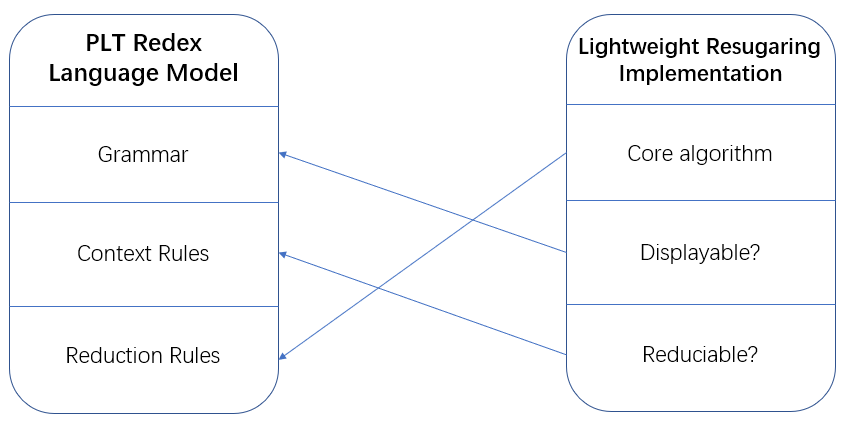
\includegraphics[width=12cm]{images/frame.png}
	\caption{framework of implementation}
	\label{fig:frame}
\end{figure}

The grammar of the whole language contains Coreexp, Surfexp and Commonexp as the language setting in sec\ref{sec3}. OtherSurfexp is of Surfexp and OtherCommonexp is of Commonexp. The identifier of any kind of expression is Headid of expression. If we need to add a syntactic sugar to the whole language, only three steps is needed.

\begin{enumerate}
\item Add grammar of the syntactic sugar.
\item Add context rules of the sugar, such that any sub-expressions can be reduced.
\item Add desugar rules of the sugar to reduction rules of the whole language.
\end{enumerate}

Then inputting an expression of the syntactic sugar to lightweight-resugaring will get the resugaring sequences.

\subsection{Evaluation}

We test some applications on the tool implemented using PLT Redex. Note that we set CBV's lambda calculus as terms in commonexp, because we need to output some intermediate sequences including lambda expressions in some examples. It's easy if we want to skip them.

\subsubsection{simple sugar}
\label{mark:simple}

We construct some simple syntactic sugar and try it on our tool. Some sugar is inspired by the first work of resugaring\cite{resugaring}. The result shows that our approach can process all sugar features of their first work.

We take a SKI combinator syntactic sugar as an example. We will show why our approach is lightweight.

\begin{flushleft}
	$S$ $\rightarrow$ $(\lambda _{N}~(x_{1}~x_{2}~x_{3})~(x_{1}~x_{2}~(x_{1}~x_{3})))$

	$K$ $\rightarrow$ $(\lambda _{N}~(x_{1}~x_{2})~x_{1})$

	$I$ $\rightarrow$ $(\lambda _{N}~(x)~x)$
\end{flushleft}

Although SKI combinator calculus is a reduced version of lambda calculus, we can construct combinators' sugar based on call-by-need lambda calculus in our CoreLang. For expression

 $(S~(K~(S~I))~K~xx~yy)$, we get the following resugaring sequences as following.
\begin{Codes}
    (S (K (S I)) K xx yy)
\CoreStep (((K (S I)) xx (K xx)) yy)
\CoreStep (((S I) (K xx)) yy)
\CoreStep (I yy ((K xx) yy))
\CoreStep (yy ((K xx) yy))
\CoreStep (yy xx)
\end{Codes}
% \begin{figure}[ht]
% 	\centering
% 	\parbox[t]{\textwidth}{
% 				\begin{center}
% 				{
% 					\small\selectfont
% 					(S (K (S I)) K xx yy)\\
% 					↓\\
% 					(((K (S I)) xx (K xx)) yy)\\
% 					↓\\
% 					(((S I) (K xx)) yy)\\
% 					↓\\
% 					(I yy ((K xx) yy))\\
% 					↓\\
% 					(yy ((K xx) yy))\\
% 					↓\\
% 					(yy xx)
% 				}
% 				\end{center}
% 			}
% 	\caption{SKI's resugaring sequences}
% 	\label{fig:SKI}
% \end{figure}

For existing approach, the sugar expression should firstly desugar to
\begin{flushleft}
$((\lambda _{N}
   (x_{1} x_{2} x_{3})
   (x_{1} x_{3} (x_{2} x_{3})))
  ((\lambda _{N} (x_{1} x_{2}) x_{1})
   ((\lambda _{N}
     (x_{1} x_{2} x_{3})
     (x_{1} x_{3} (x_{2} x_{3})))
    (\lambda _{N} (x) x)))
  (\lambda _{N} (x_{1} x_{2}) x_{1})
  xx
  yy)$
\end{flushleft}

Then in our CoreLang, the execution of expanded expression will contain 33 steps. For each step, there will be many attempts to match and substitute the syntactic sugars. We will omit more steps for a larger expression. So the unidirectional resugaring algorithm makes our approach lightweight.todo

\subsubsection{hygienic macro}
\label{mark:hygienic}

The second work\cite{hygienic} mainly processes hygienic macro compared to first work. We try a $Let$ sugar , which is a common hygienic sugar example, on our tool. Our algorithm can easily process hygienic macro without special data structure. The $Let$ sugar is define as follow

$(Let\;x\;v\;exp)$ $\rightarrow$ $(Apply\;(\lambda\;(x)\;exp)\;v)$

Take $(Let~x~1~(+~x~(Let~x~2~(+~x~1))))$ for an example. First, a temp expression

$(Apply\;(\lambda\;(x)\;(+~x~(Let~x~2~(+~x~1))))\;1)$

is needed. (case 5 or 6)Then one-step try on the temp expression, we will get

$(+~1~(Let~1~2~(+~1~1)))$ which is out of the whole language's grammar. In this case, it is not a good choice to desugar the outermost $Let$ sugar. Then we just apply the core-algo f on the sub-expression where the error occurs ($(+~x~(Let~x~2~(+~x~1)))$ in this example). So the right intermediate sequence $(Let~x~1~(+~x~3))$ will be get.

In practical application, we think resugaring for a unhygienic rewriting system is not interesting at all, because hygienic macro can be easily processed by rewriting system. So in the finally implementation of our tool, we just use PLT Redex's binding forms to deal with hygienic macros. But we did try it on the version without hygienic rewriting system.

\subsubsection{recursive sugar}
Recursive sugar is a kind of syntactic sugars where call itself or each other during the expanding. For example,

$(Odd\;e)$ $\rightarrow$ $(if\;(>\;e\;0)\;(Even\;(-\;e\;1)\;\#f))$

$(Even\;e)$ $\rightarrow$ $(if\;(>\;e\;0)\;(Odd\;(-\;e\;1)\;\#t))$

are typical recursive sugars. The previous works can process this kind of syntactic sugar easily, because boundary conditions are in the sugar itself.

Take $(Odd~2)$ as an example. The previous work will firstly desugar the expression using the rewriting system. Then the rewriting system will never start resugaring as Fig\ref{fig:odd} shows.

\begin{figure}[ht]
	\centering
	\parbox[t]{\textwidth}{
				\begin{center}
				{
					\small\selectfont
					(Odd 2)\\
					↓\\
					(if (> 2 0) (Even (- 2 1) \#f))\\
					↓\\
					(if (> (- 2 1) 0) (Odd (- (- 2 1) 1) \#t))\\
					↓\\
					(if (> (- (- 2 1) 1) 0) (Even (- (- (- 2 1) 1) 1) \#f))\\
					↓\\
					{\ldots}
				}
				\end{center}

			}
	\caption{Odd2's desugaring process}
\label{fig:odd}
\end{figure}

Then the advantage of our approach is embodied. Our lightweight approach doesn't require a whole expanding of sugar expression, which gives the framework chances to judge boundary conditions in sugars themselves, and showing more intermediate sequences. We get the resugaring sequences as Fig \ref{fig:rec} of the former example using our tool.

\begin{figure}[ht]
	\centering
	\parbox[t]{\textwidth}{
				\begin{center}
				{
					\small\selectfont
					(Odd 2)\\
					↓\\
					(Even (- 2 1))\\
					↓\\
					(Even 1)\\
					↓\\
					(Odd (- 1 1))\\
					↓\\
					(Odd 0)\\
					↓\\
					\#f
				}
				\end{center}

			}
	\caption{Odd2's resugaring sequences}
\label{fig:rec}
\end{figure}

We also construct some higher-order syntactic sugars and test them. The higher-order feature is important for constructing practical syntactic sugar. And for syntactic sugar's feature, it is of recursive sugar. Giving the following two higher-order syntactic sugar as examples.

\begin{flushleft}
	$(map\;e\;(list\;v_1\ldots))$→

	$(if\;(empty\;(list\;v_1\ldots))\;(list)\;(cons\;(e\;(first\;(list\;v_1\ldots)))\;(map\;e\;(rest\;(list\;v_1\ldots)))))$
\end{flushleft}

\begin{flushleft}
	$(filter\;e\;(list\;v_1\;v_2\ldots))$→

	$(if\;(e\;v_1)\;(cons\;v_1\;(filter\;e\;(list\;v_2\ldots)))\;(filter\;e\;(list\;v_2\ldots)))$

	$(filter\;e\;(list))$ → $(list)$
\end{flushleft}
These two syntactic sugars use different sugar forms to implement. For $Map$ sugar, we use if expression in CoreLang to constrain the boundary conditions. For $Filter$ sugar, we use two different parameters' form, which is another easy way for constructing syntactic sugar. The testing results show as Fig\ref{fig:map} \ref{fig:filter}.

\begin{figure}[ht]
	\centering
	\parbox[t]{\textwidth}{
				\begin{center}
				{
					\small\selectfont
					(map (λ (x) (+ 1 x)) (list 1 2 3))\\
					↓\\
					(cons 2 (map (λ (x) (+ 1 x)) (list 2 3)))\\
					↓\\
					(cons 2 (cons 3 (map (λ (x) (+ 1 x)) (list 3))))\\
					↓\\
					(cons 2 (cons 3 (cons 4 (map (λ (x) (+ 1 x)) (list)))))\\
					↓\\
					(cons 2 (cons 3 (cons 4 (list))))\\
					↓\\
					(cons 2 (cons 3 (list 4)))\\
					↓\\
					(cons 2 (list 3 4))\\
					↓\\
					(list 2 3 4)
				}
				\end{center}

			}
	\caption{Map's resugaring sequences}
\label{fig:map}
\end{figure}

\begin{figure}[ht]
	\centering
	\parbox[t]{\textwidth}{

				\begin{center}
				{
					\small\selectfont
					(filter (λ (x) (and (> x 3) (< x 6))) (list 1 2 3 4 5 6 7))\\
					↓\\
					(filter (λ (x) (and (> x 3) (< x 6))) (list 2 3 4 5 6 7))\\
					↓\\
					(filter (λ (x) (and (> x 3) (< x 6))) (list 3 4 5 6 7))\\
					↓\\
					(filter (λ (x) (and (> x 3) (< x 6))) (list 4 5 6 7))\\
					↓\\
					(cons 4 (filter (λ (x) (and (> x 3) (< x 6))) (list 5 6 7)))\\
					↓\\
					(cons 4 (cons 5 (filter (λ (x) (and (> x 3) (< x 6))) (list 6 7))))\\
					↓\\
					(cons 4 (cons 5 (filter (λ (x) (and (> x 3) (< x 6))) (list 7))))\\
					↓\\
					(cons 4 (cons 5 (filter (λ (x) (and (> x 3) (< x 6))) (list))))\\
					↓\\
					(cons 4 (cons 5 (list)))\\
					↓\\
					(cons 4 (list 5))\\
					↓\\
					(list 4 5)
				}

				\end{center}

			}
	\caption{Filter's resugaring sequences}
\label{fig:filter}
\end{figure}
\subsection{Compare to previous work}

As mentioned many times before, the biggest difference between previous resugaring approach and our approach, is that our approach doesn't need to desugar the sugar expresssion totally. Thus, our approach has the following advantages compared to previous work.

\begin{itemize}
	\item {\bfseries Lightweight} As the example at sec\ref{mark:simple}, the match and substitution process searchs all intermediate sequences many times. It will cause huge cost for a large program. So out approach---only expanding a syntactic sugar when necessarily, is a lightweight approach.
	\item {\bfseries Friendly to hygienic macro} Previous hygienic resugaring approach use a new data structure---abstract syntax DAG, to process resugaring of hygienic macros. Our approach simply finds hygienic error after expansion, and gets the correct reduction instead.
	\item {\bfseries More syntactic sugar features} The ability of processing recursive sugar is a superiority compared to previous work. The key point is that recursive syntactic sugar must handle boundary conditions. Our approach handle them easily by not necessarily desugaring all syntactic sugars. Higher-order functions, as an important feature of functional programming, was supported by many daily programming languages. So the ability on higher-order sugar is important.
	\item {\bfseries Rewriting rules based on reduction semantics} Any syntactic sugar that can expressed by reduction semantics can be used in our approach. It will give more possible forms for constructing syntactic sugars. todo:example?
\end{itemize}

%!TEX root = ./main.tex
\section{Derivation of Evaluation Rules}
\label{sec:ruleDerivation}

So far, we have shown that our resugaring algorithm can use lazy desugaring to avoid costive reverse desugaring in the traditional approach. However, as shown in the reduction rules {\sc SurfRed1} and {\sc SurfRed2}, we still need a one-step try to check whether a syntactic sugar is required or not. It would be more efficient if such one-step try could be avoided. In this section, we show that this is possible, by giving an automatic method to derive evaluation rules for the syntactic sugar through symbolic computation.
%As demonstrated in Section \ref{sec2}, this will significantly improve the efficiency of our resugaring.
%In this section, we purpose such a method to make the resugaring of syntactic sugar more efficient.

%As discussed in the overview, frequent attempts on reverse desugaring during traditional resugaring processes is costive and inefficient. If we can statically derive syntactic sugar's evaluation rules through its structure, it will greatly improve the efficiency of resugaring. In this section, we purpose such a method to make the resugaring of syntactic sugar more efficient.

To see our idea, consider a simple syntactic sugar defined by $\drule{(\m{Not}~e_1)}{(\m{if}~e_1~\m{\#f}~\m{\#t})}$. To derive reductions rules for \m{not} from those of \m{if}, we design \textit{inference automaton} (IFA) that can be used to express and manipulate a set of evaluation rules for a language construct.
%
Assuming that we already have the IFAs of all language constructs of the core language, our method to construct the evaluation rules of a syntactic sugar is as follows: First, we construct an IFA for the syntactic sugar according to the desugaring rules, then we transform and simplify the IFA, and finally we generate evaluation rules for the syntactic sugar from the IFA.

In this following, we start with some examples of IFA, its formal definition and its normal form, before we proceed to give our algorithm for conversion between evaluation rules and IFA.
%We discuss the role of IFA in dealing with syntactic sugar.

\subsection{Inference Automaton}

As mentioned above, IFA intuitively describes the evaluation rules of a certain language construct. To help readers better understand it, we start with some examples, then we give the formal definition of IFA.

\begin{example}[IFA of~~ \m{if}]

    Recall the three evaluation rules of \m{if} in the overview. Given an expression \Code{(if $e_1$ $e_2$ $e_3$)}, from these rules, we can see that $e_1$ should be evaluated first, then $e_2$ or $e_3$ will be chosen to evaluate depending on the value of $e_1$. The evaluation result of $e_2$ or $e_3$ will be the value of the expression. This evaluation procedure (or the three evaluation rules) for \Code{(if $e_1$ $e_2$ $e_3$)} can be represented by the IFA in Figure \ref{fig:ifa-if}.

    \begin{figure}[t]
        \centering
        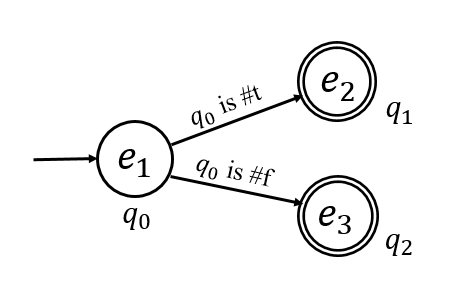
\includegraphics[scale=0.25]{images/ifa/ifa-if.png}
        \caption{IFA of \m{if}}
        \label{fig:ifa-if}
    \end{figure}

    A node of IFA indicates that the expression needs to be evaluated, and the nodes before it have been evaluated. The arrow from $q_0$ to $q_1$ indicates that this branch is selected when the evaluation result of $e_1$ is \m{\#t}. The arrow between $e_1$ and $e_3$ is similar. The double circles of $e_2$ and $e_3$ denote that their evaluation result will be the result of the expression with this language construct. In most cases, the transition condition is the evaluation result (an abstract value) of the previous node or a specific value, so to simplify the representation of IFA, we will only mark the value on the transition edge when it is clear from the context.

    When an expression with \m{if} needs to be evaluated (for example \m{(if (if \#t \#t \#f) \#f \#t)}), first evaluating the $e_1$ (\m{(if \#t \#t \#f)}). Note that in this process, evaluating a subexpression requires running another automaton based on its syntax, while the outer automaton hold the state at $q_0$. According to the result of $e_1$ (which is \m{\#f} in this case), the IFA selects the branch ($e_3$). Then the result of $e_3$ (\m{\#t}) is the evaluation result of the expression.
    \myend
\end{example}

\begin{example}[IFA of \m{nand}]

    \begin{figure}[t]
        \centering
        \subcaptionbox{IFA according to the rules \label{fig:ifa-nand-a}}[.31\linewidth]{
            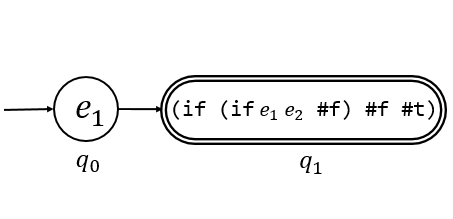
\includegraphics[scale=0.25]{images/ifa/ifa-nand-1-small.png}
        }
        \subcaptionbox{After expanding the outer \m{if} \label{fig:ifa-nand-b}}[.31\linewidth]{
            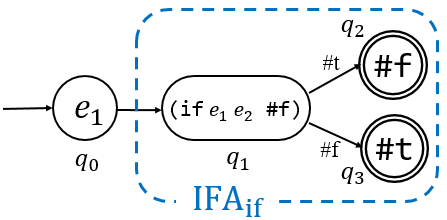
\includegraphics[scale=0.25]{images/ifa/ifa-nand-2-small.png}
        }
        \subcaptionbox{After expanding the inner \m{if} \label{fig:ifa-nand-c}}[.33\linewidth]{
            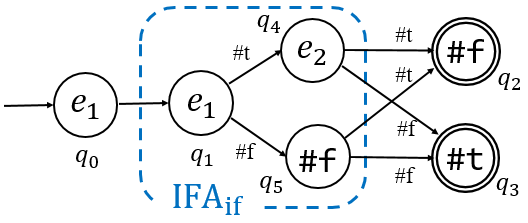
\includegraphics[scale=0.25]{images/ifa/ifa-nand-3-small.png}
        }
        \caption{IFA of \m{nand}}
        \label{fig:ifa-nand}
    \end{figure}

    Sometimes the rules may be more complex, such as being reduced into another language construct, or an expression containing other syntactic structures. For example, for the following evaluation rules for \m{nand}:
    \[
        \infer{(\m{nand}~e_1~e_2) \to (\m{nand}~e_1'~e_2)}{e_1 \to e_1'}
    \]\[
        (\m{nand}~v_1~e_2) \to (\m{if}~(\m{if}~v_1~e_2~\m{\#f})~\m{\#f}~\m{\#t})
    \]
    %
    % \infrule[E-Nand]{e_1 \to e_1'}{(\m{nand}~e_1~e_2) \to (\m{nand}~e_1'~e_2)}
    % \infax[E-NandV]{(\m{nand}~v_1~e_2) \to (\m{if}~(\m{if}~v_1~e_2~\m{\#f})~\m{\#f}~\m{\#t})}
    %
    we can draw \m{nand}'s IFA as Figure \ref{fig:ifa-nand-a}.
    When the automaton runs into the terminal node of Figure \ref{fig:ifa-nand-a}, it goes to derive the \m{if} expression. In fact, we have known how \m{if} works through the IFA of \m{if}. Thus we can replace the last node with an $\text{IFA}_{\m{\scriptsize if}}$ and substitute $e_1$ to $e_3$ of $\text{IFA}_{\m{\scriptsize if}}$ with the parameters of the node. Use the termination nodes of $\text{IFA}_{\m{\scriptsize if}}$ as the termination nodes of new $\text{IFA}_{\m{\scriptsize \scriptsize nand}}$. The results are shown in Figure \ref{fig:ifa-nand-b}. Further decomposing the inner \m{if} node, connecting the terminating nodes of $\text{IFA}_{\m{\scriptsize nand}}$ to the nodes pointed to by the original output edge, we get Figure \ref{fig:ifa-nand-c}.

    As the nodes of IFA in Figure \ref{fig:ifa-nand-c} have no other composite syntactic structures, such an IFA completely expresses the semantics of a language construct, and no longer cares about the evaluation rules of other syntactic structures. We will do similar steps for syntactic sugars, which will be discussed later.
    \myend
\end{example}

\begin{example}[IFA of \m{and}]

    Suppose that the evaluation rule of \m{and} is defined in a more complex way as follows.
    \[
        (\m{and}~e_1~e_2) \to (\m{let}~x~e_1~(\m{if}~x~e_2~x))
    \]
    In this case, we use the let binding, and we introduce a symbol table to record the bindings between variables and expressions (corresponding to nodes). The representation of $\text{IFA}_{\m{\scriptsize and}}$ is shown in Figure \ref{fig:ifa-and-a}.

    Further discuss the language construct. We first evaluate $e_1$ and save the result in $x$. When evaluating the expression of \m{if}, what is actually evaluated is $(\m{if}~x~e_2~x)[e_1/x]$. We represent it in the form of Figure \ref{fig:ifa-and-b}, where node $q_1$ contains a symbol table for recording the mapping from variables to nodes.
    %It is similar to context, but since we map the variable to the node, we distinguished it.
    Mapping to nodes is to ensure that the variable information will not be lost when the IFA is transformed.
    \myend
\end{example}


\begin{figure}[t]
    \centering
    \subcaptionbox{IFA according to the rules \label{fig:ifa-and-a}}[.4\linewidth]{
        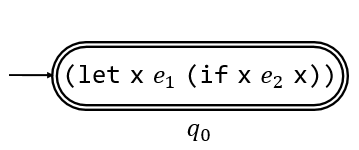
\includegraphics[scale=0.25]{images/ifa/ifa-and-1.png}
    }
    \subcaptionbox{After expanding \m{let} \label{fig:ifa-and-b}}[.4\linewidth]{
        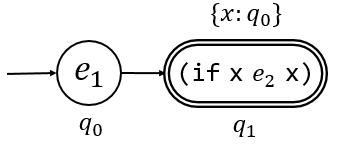
\includegraphics[scale=0.25]{images/ifa/ifa-and-2.png}
    }
    \caption{IFA of \m{and}}
    \label{fig:ifa-and}
\end{figure}

%--------------------------------
%\subsubsection{Definition of IFA}

\begin{Def}[Inference Automaton]

    An inference automaton (IFA) of language construct \m{H} is a 5-tuple, $(Q, \Sigma, q_0, F, \delta)$, consisting of

    \begin{itemize}
        \item A finite set of nodes $Q$, each node containing an expression and a symbol table which maps a variable to a node;
        \item A finite set of conditions $\Sigma$;
        \item A start node $q_0 \in Q$;
        \item A set of terminal nodes $F \subseteq Q$; and
        \item A transition function $\delta: (Q-F) \times \Sigma' \to Q$ where $\Sigma' \subseteq \Sigma$.
    \end{itemize}
    and for each node $q$, there is no path to itself (i.e., there is no sequence of conditions $C = (c_1,c_2,\ldots,c_n)\subseteq \Sigma^*$, such that after $q$ transfers sequentially according to $P$, it returns $q$.)

\end{Def}

%The last constraint requires that there be no circles in our IFA.
The state transition depends on whether the expression meets the condition. Note that each IFA is associated with language construct. Each state in IFA represents the current evaluation of a language construct, indicating that some subexpressions of the language construct have been evaluated at this state, and the rest have not.

%======================
\subsection{Normal IFA}

Although IFA can describe the evaluation behavior of a language construct, IFA itself may be in a complicated form. For example, the IFA of a language construct contains other syntactic structures in Figure \ref{fig:ifa-nand-a}. We will simplify IFA to make it easier to analyze.

\begin{Def}[Normal IFA]
    \label{def:nmlifa}
    An IFA is said to be normal if it satisfies the following conditions.
    \begin{itemize}
        \item The expression of node $q \in Q$ can only be a pattern variable $e_i$ or a local variable $x$. If it is a local variable, it cannot be in the symbol table of $q$.
        \item For any $q_1,q_2 \in Q$ and $c_1, c_2 \in \Sigma$, $\delta(q_1, c_1) \neq \delta(q_2, c_2)$.
        \item On each branch, each pattern variable $e_i$ can only be evaluated once.
    \end{itemize}
\end{Def}

If an IFA is normal, it means that there are no more composite syntactic structures in it, and that it is of a tree structure.
In fact, it is always feasible to convert IFA to normal IFA.

\begin{mythm}[Normalizability of IFA]
    \label{mythm:nmlifa}
    An IFA can be transformed into a normal IFA, if the normal IFAs of all sub-syntactic structures in the IFA are known.
\end{mythm}

We can prove this theorem by repeatedly applying the following correctness-preserving steps to normalize an IFA.
% and prove their correctness.

%------------------------------------
\subsubsection*{Step 1: Transforming into a Tree}

As we have assumed that evaluation of a subexpression does not have side effect on the evaluation of other subexpressions, a node with at least two sources can be cloned and applied to different branches as shown in Figure \ref{fig:nmlifa-tree}; replacing the node referenced by the branch with the cloned node in conditions and symbol tables.  In this way, we can transform an IFA into a tree so that it meet the second condition for a  normal IFA.

\begin{figure}[t]
    \centering
    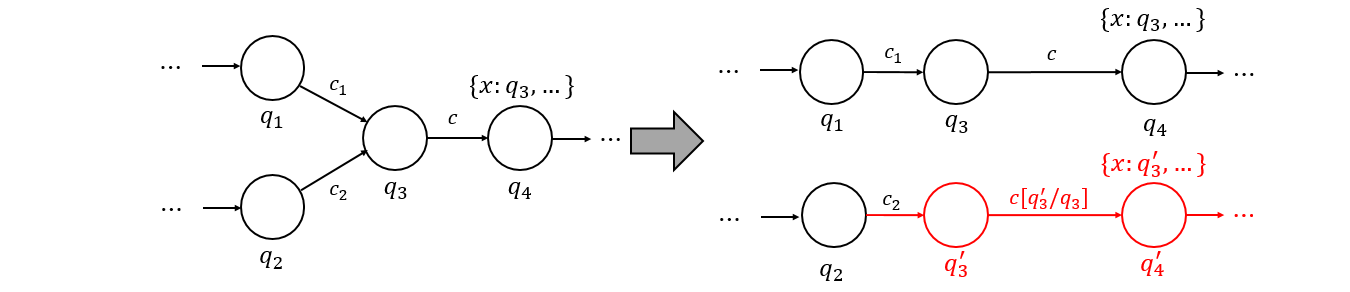
\includegraphics[scale=0.25]{images/nmlifa/nmlifa-tree.png}
    \caption{Transform into a Tree}
    \label{fig:nmlifa-tree}
\end{figure}

%-------------------------------------------------
\subsubsection*{Step 2: Substituting Sub-Language Construct}
\label{mark:hygieneinderive}

If node $q$ in the tree IFA contains an expression of a language construct \m{H}, we replace this node with the normal IFA of \m{H}, replace the parameters, and pass the symbol table of $q$ into the sub-IFA. Then, connect all the termination nodes of \m{H} to the original output node $q'$, and convert it into a tree IFA according to the method described in the previous step as shown in Figure \ref{fig:nmlifa-subst}. Replace the node referenced by the branch with the \textit{new} one in conditions and symbol tables. This step preserve the semantics because of $(\m{H}~e_1~\ldots~e_n)[e/x] = (\m{H}~e_1[e/x]~\ldots~e_n[e/x])$.

In particular, if an expression $e$ does not contain a certain variable $x$, we can remove it from the symbol table. For example, in our problem, each pattern variable $e_i$ of syntactic sugar cannot contain unbound variables. So we can remove all symbol tables of nodes with $e_i$.

Note that even for hygienic sugar, this step of substitution is correct. Because what we require to substitute is a normal IFA, if the expression of a node $q$ in sub-IFA is a local variable $x$, it must be unknowable in the substructure ($x$ not in the symbol table of $q$). So the value of $x$ must be passed from the outer language construct.

\begin{figure}[t]
    \centering
    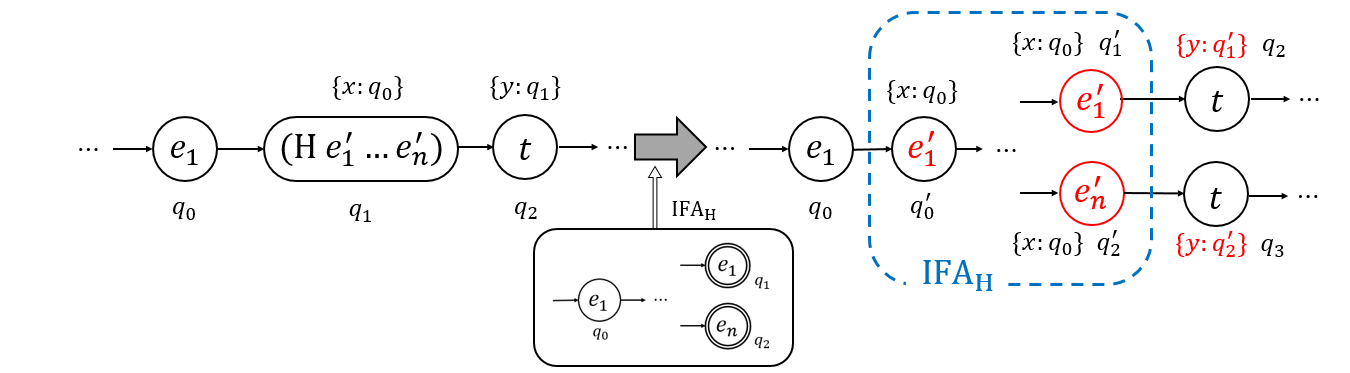
\includegraphics[scale=0.25]{images/nmlifa/nmlifa-subst.png}
    \caption{Substitute Sub-Language Construct}
    \label{fig:nmlifa-subst}
\end{figure}

%----------------------------------------------------
\subsubsection*{Step 3: Replacing Variables in the Symbol Table}

If the expression of a node $q$ is a local variable $x$ and $x$ is in the symbol table of $q$, we can replace $x$ with the expression of the node it points to, then remove $x$ from the symbol table as shown Figure \ref{fig:nmlifa-replace}. Because $x[e_1/x, e_2/y]=e_1[e_2/y]$, this step is correct.

\begin{figure}[t]
    \centering
    
\includegraphics[scale=0.25]{images/nmlifa/nmlifa-replace.png}
    \caption{Replace Variables in the Symbol Table}
    \label{fig:nmlifa-replace}
\end{figure}

%---------------------------------------------------------------------
\subsubsection*{Step 4: Removing Evaluated Nodes and Merge Transition Conditions}

If an IFA is a tree, for each branch, remove the non-terminal nodes that have been evaluated with the same symbol table, and merge the conditions on the transition edge as in Figure \ref{fig:nmlifa-merge}. Replace the node referenced by the branch with the first-evaluated node in conditions and symbol tables. This step can make an IFA satisfy the third constraint of normal IFA.

Since on any branch, if $e_i$ is removed, it must have been evaluated. Therefore, when IFA runs to this node, there is no need to do any evaluation on $e_i$. At the same time, the transfer edge ensures that the conditions are not lacking. Correctness is guaranteed.

\begin{figure}[t]
    \centering
    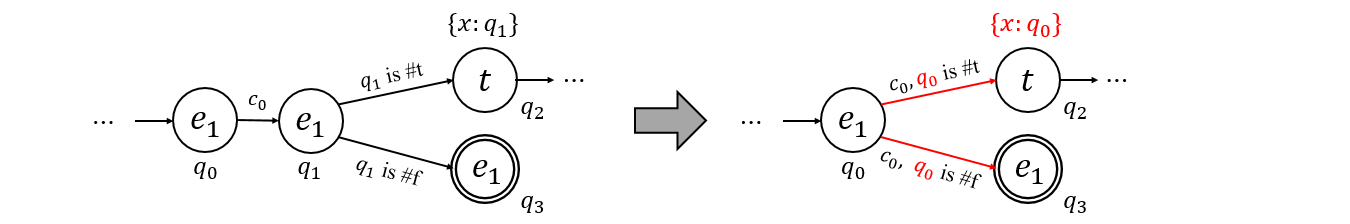
\includegraphics[scale=0.25]{images/nmlifa/nmlifa-merge.png}
    \caption{Remove Evaluated Nodes and Merge Transition Conditions}
    \label{fig:nmlifa-merge}
\end{figure}

%------------------------------------
\subsubsection*{Step 5: Removing Constant Value}

If the expression of a node is a constant value, remove the node and merge the conditions on the transition edge just like evaluated value. Because IFA does not do anything in this node, this does not affect the correctness of IFA.

%-------------------------------------
%\subsubsection{Normalizability of IFA}

%\begin{proof}[Proof of Theorem \ref{mythm:nmlifa}]
%    By repeating the above steps continuously, we can always get normal IFA. And it is equivalent to the original IFA for the correctness of each step.
%\end{proof}

%===========================================
\subsection{Converting Evaluation rules to IFA}

At the beginning of this section, we have shown several examples about correspondence between IFA and evaluation rules. Now, we give an algorithm that can automatically convert the evaluation rules to IFA and ensure its correctness. But at the same time, it has stricter requirements on the evaluation rules.

In this section, we only discuss core language. Syntactic sugar is similar to this, which we discuss it later.

%--------------------------
%\subsubsection{Assumptions}

\begin{Asm}
    \label{Asm:rules}
    A language construct $H$ only contains the evaluation rules in the following form:
    \[
        \infer
        {(\m{H}~e_1 \ldots e_i \ldots e_n) \to (\m{H}~e_1 \ldots e_i' \ldots e_n)}{e_i \to e_i'\quad T}
    \]
    \[
        \infer{(\m{H}~v_1 \ldots v_p~e_1 \ldots e_q) \to e}{T}
    \]
    %where $e$ can be any value, one of the parameters or a term of another language construct.
    where $T$ is a constraint over $e_j$ for $j \in 1,2,\ldots,n$.
\end{Asm}

This assumption specifies the form of the evaluation rules to ensure that IFAs can be generated. The first one is a context rule, and the other one is a reduction rule. Rule $(\m{if}~\m{\#t}~e_1~e_2) \to e_1$ can be seen as \[\infer{(\m{if}~e~e_1~e_2) \to e_1}{e~\key{is}~\m{\#t}}.\]

\begin{Asm}[Orderliness of Language Construct]
    \label{Asm:orderliness}
    The language construct in the core language is finite. Think of all syntactic structures as points in a directed graph. If one of $H$'s evaluation rules can generate an expression containing $H'$, then construct an edge that points from $H$ to $H'$. The directed graph generated in this method has no circles.
\end{Asm}

IFAs are not able to construct syntactic structures that contain recursive rules. This assumption qualifies that we can find an order for all syntactic structures, and when we try to construct IFA for $H$, IFA of $H'$ is known.

\begin{Asm}[Determinacy of One-Step Evaluation]
    \label{Asm:determinacy}
    The evaluation rules satisfy the determinacy of one-step evaluation.
\end{Asm}

By assumption \ref{Asm:determinacy}, we can get the following lemma, which points out the feasibility of using a node in IFA to represent the evaluation of subexpressions.

\begin{lemma}
    \label{lemma:one-step}
    If an expression $(\m{H}~e_1~\ldots~e_n)$ does a one-step evaluation by a context rule, which is a one-step evaluation of pattern variable $e_i$, then it continues to use this rule until $e_i$ becomes a value.
\end{lemma}

\begin{proof}[Proof of Lemma \ref{lemma:one-step}]
    According to Assumption \ref{Asm:determinacy}, this lemma is trivial.
\end{proof}

%------------------------
\subsubsection{Converting Algorithm}

\begin{mythm}[IFA Can Be Constructed by Evaluation Rules]
    \label{mythm:Rule2IFA}
    If all the syntactic structures in the core language satisfy these assumptions, we can construct IFAs for all syntactic structures in the core language.
\end{mythm}

\begin{proof}[Proof of Theorem \ref{mythm:Rule2IFA}]

    We prove this theorem by giving an algorithm that converts evaluation rules to IFA. By Assumption \ref{Asm:orderliness}, we get an order of syntactic structures. We construct the IFA for each structure in turn.

    We generate a node for each rule of the language construct \m{H} and insert them into $Q$. If the rule is a context rule for a pattern varibale $e_i$, set $e_i$ as the expression of the node. If the rule is a reduction rule, add them into $F$ as terminal nodes and set the reduced expression $e$ as the expression of the node. Symbol tables of these nodes are set to be empty. Next we connect these nodes.

    For an expression like $(\m{H}~e_1~\ldots~e_n)$, suppose that $e_1, \ldots, e_n$ are not value, According to Lemma \ref{lemma:one-step}, we have the unique rule $r$ of \m{H} for one-step evaluation. Let node $q$ corresponding to $r$ be $q_0$.

    If $r$ is a context rule for $e_i$, let the expression of $q$ be $e_i$. Assume that the evaluation of $e_i$ results in $v_i$, we get expression $(\m{H}~e_1 \ldots e_{i-1}~v_i~e_{i+1} \ldots e_n)$. For each possible value of $v_i$, choose the rules $r'$ that should be used. The node is $q'$. Set a condition as $c=q~\key{is}~v_i$ Let $\delta(q, c)$ be $q'$. For each branch, seem $r'$ as $r$ and keep doing this until $r$ is a reduction rule.
\end{proof}

In this way, we got an IFA of \m{H}. According to the lemma \ref{mythm:nmlifa}, we can also get a normal IFA of \m{H}.

%---------------------------------------------------------
\begin{example}[Constructing IFA of \m{xor} by Rules]

    We give an example to show how to convert evaluation rules to IFA using the algorithm mentioned above. Since the symbol tables of all nodes are empty, we omit not to write.

    \infrule[E-Xor]{e_1 \to e_1'}{(\m{xor}~e_1~e_2) \to (\m{xor}~e_1'~e_2)}
    \infax[E-XorTrue]{(\m{xor}~\m{\#t}~e_2) \to (\m{if}~e_2~\m{\#f}~\m{\#t})}
    \infrule[E-XorFalse]{e_2 \to e_2'}{(\m{xor}~\m{\#f}~e_2) \to (\m{xor}~\m{\#f}~e_2')}
    \infax[E-XorFalseTrue]{(\m{xor}~\m{\#f}~\m{\#t}) \to \m{\#t}}
    \infax[E-XorFalseFalse]{(\m{xor}~\m{\#f}~\m{\#f}) \to \m{\#f}}

    Suppose that \m{xor} is a language construct in core language. There are five rules for it. Therefore, we construct five nodes for the rules and set the expression as Figure \ref{fig:ifa-xor-a}.

    Considering an expression $(\m{xor}~e_1~e_2)$, where $e_1$ and $e_2$ are not values. It will be derived by rule (E-Xor). Therefore, set the node of the rule as the start node $q_0$. According to the rules of \m{xor}, the evaluation result of $e_1$ can be \m{\#t} or \m{\#f}. If the value is \m{\#t}, the expression will be $(\m{xor}~\m{\#t}~e_2)$ and use rule (E-XorTrue) to derive. Then connect $q_0$ and $q_1$ with condition $q_0~\key{is}~\m{\#t}$. Connect $q_0$ and $q_2$ with condition $q_0~\key{is}~\m{\#f}$ similarly as Figure \ref{fig:ifa-xor-b}. Then connect $q_2$ to the last two nodes with conditions according to the value of $e_2$. The IFA of \m{xor} can be expressed as Figure \ref{fig:ifa-xor-c}.
    \myend
\end{example}

\begin{figure}[t]
    \centering
    \subcaptionbox{\label{fig:ifa-xor-a}}[.3\linewidth]{
        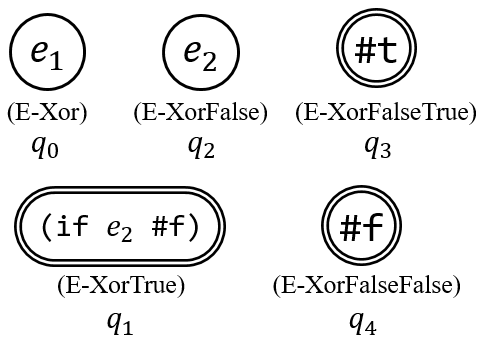
\includegraphics[scale=0.22]{images/ifa/ifa-xor-1.png}
    }
    \subcaptionbox{\label{fig:ifa-xor-b}}[.33\linewidth]{
        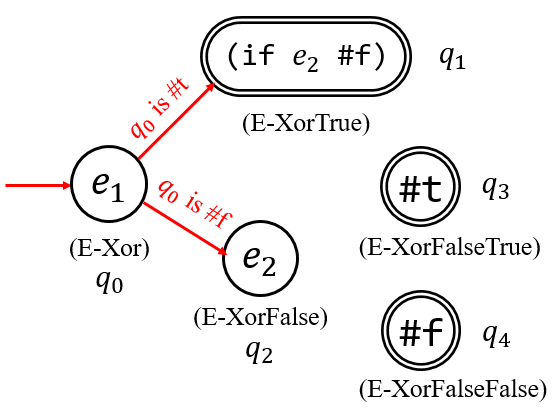
\includegraphics[scale=0.22]{images/ifa/ifa-xor-2.png}
    }
    \subcaptionbox{\label{fig:ifa-xor-c}}[.33\linewidth]{
        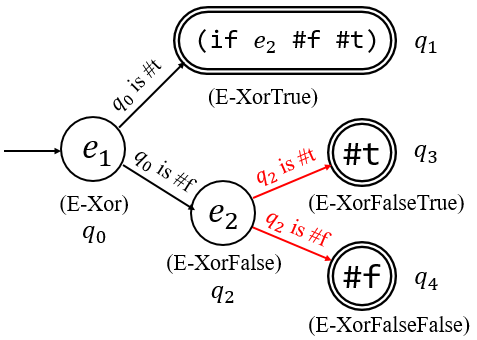
\includegraphics[scale=0.22]{images/ifa/ifa-xor-3.png}
    }
    \caption{IFA of \m{xor}: Constructed by evaluation rules}
    \label{fig:ifa-xor}
\end{figure}

%--------------------------
\subsubsection{Correctness}
~\\

Before proving the correctness of the algorithm, we first prove the following lemma.

\begin{lemma}
    \label{lemma:accessibility}
    If an expression $e$ of language construct \m{H} uses rule $r$ to derive, we can find a path from $q_0$ to $q$ generated by $r$.
\end{lemma}

\begin{proof}[Proof of Lemma \ref{lemma:accessibility}]
    Suppose $e=(\m{H}~v_1~\ldots~v_p~e_1~\ldots~e_q)$. We build an expression $e_0'=(\m{H}~\m{id}(v_1)~\ldots~\m{id}(v_p)~e_1~\ldots~e_q)$, where $\m{id}(x)=x$. $e_0'$ should have the same value as $e$. If $e_0'$ is derived by rule $r_1$, $r_1$ must be a context rule, or $e$ can also be reduced by $r_1$. Also, the node $q_1$ generated by $r_1$ will be the start node. Without loss of generality, assume that $r_1$ is a context rule for $e_1$. We get $e_1'=(\m{H}~v_1~\m{id}(v_2)~\ldots~\m{id}(v_p)~e_1~\ldots~e_q)$ after derived by $r_1$. Similarly, we find a rule $r_2$ which is a context rule for $e_2$. The node $q_2$ generated by $r_2$ satisfies $\delta(q_1, (e_1~\key{is}~v_1))=q_2$. By analogy, we can get $e_p'=(\m{H}~v_1~\ldots~v_p~e_1~\ldots~e_q)=e$ and a path $q_1(=q_0), q_2, \ldots, q_p$. At last, we use rule $r$ to derive $e$ and add $q$ to the path.
\end{proof}

\begin{lemma}[Correctness]
    \label{lemma:rule2ifa-correct}
    For any language construct \m{H}, under our assumption, the normal IFA got by the algorithm in Theorem \ref{mythm:Rule2IFA} has the same semantics as the rules.
\end{lemma}

%In other words, for any term of language construct \m{H}, evaluating the term by IFA and evaluating by rule get the same derivation sequence.

\begin{proof}
    %[Proof of Lemma \ref{lemma:rule2ifa-correct}]
    We only need to discuss that in a one-step derivation, both get the same result.

    Consider an expression $e=(\m{H}~e_1 \ldots e_n)$ and a rule $r$ for derivation. Suppose $r$ generates node $q$. By Lemma \ref{lemma:accessibility}, we find a path from $q_0$ to $q$. The expression $e$ must meet the conditions from $q_0$ to $q$. Therefore, the one-step derivation of this expression $e$ in IFA must be located at $q$. If $r$ is a context rule for a pattern variable $e_i$, the expression of $q$ is $e_i$ as well, and $e_i$ of $e$ is not a value. Thus both of the one-step derivation of $e$ are one-step derivation of $e_i$. If $r$ is a reduction rule to $e'$, both are $e'$.

    Similarly, if an expression can be derived in one step in IFA, then it must be able to use the corresponding rule for one-step derivation.
\end{proof}

%-----------------------------
%\subsubsection{IFA of \m{let}}

It should be noted that if a certain language construct does not meet our assumptions, it does not mean that this language construct does not have an IFA. We can define its IFA according to its semantics. However, this method cannot be automated and requires users to ensure its correctness. For example, given the evaluation rules of \m{let}, we can specify the IFA of \m{let} as Figure \ref{fig:ifa-let}.
\[
    \infer{\m{let}~x~e_1~e_2 \to \m{let}~x~e_1'~e_2}{e_1 \to e_1'}
\]\[
    (\m{let}~x~e_1~e_2) \to e_2[e_1/x]
\]

% \infrule[E-Let]{e_1 \to e_1'}{\m{let}~x~e_1~e_2 \to \m{let}~x~e_1'~e_2}
% \infax[E-LetSubst]{(\m{let}~x~e_1~e_2) \to e_2[e_1/x]}

\begin{figure}[t]
    \centering
    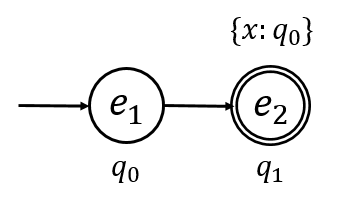
\includegraphics[scale=0.25]{images/ifa/ifa-let.png}
    \caption{IFA of \m{let}}
    \label{fig:ifa-let}
\end{figure}

In the evaluation rules of \m{let}, there is a substitution. Therefore, in IFA of \m{let}, we need symbol table to express this. When $e_2$ is evaluated or expanded, it is necessary to replace $x$ with the value of node $q_0$ in $e_2$.




%===========================================
\subsection{Converting IFA to Evaluation Rules}

Next we show how to convert IFA back to evaluation rules. Because IFA can be normalized by Theorem \ref{mythm:nmlifa}, we only need to convert normal IFA into rules. Unfortunately, IFA can express some derivation methods whose evaluation rules are difficult to describe. Therefore, we have to impose more constraints on IFA to ensure that evaluation rules can be automatically generated.

\begin{Asm}
    \label{Asm:st}
    In a normal IFA, if $q \notin F$, then the symbol table of $q$ is empty, and the expression of $q$ cannot be a local variable.
\end{Asm}

In fact, this is a strong assumption, which requires that only terminal nodes could have substitution. This is because it is difficult to generate a context rule for an expression after its substitution.

%------------------------
\subsubsection{Algorithm}

Similarly, we first give its algorithm, and then prove its correctness.

\begin{mythm}[Rules Can Be Constructed by Normal IFA]
    \label{mythm:ifa2rule}
    For each normal IFA satisfy Assumption \ref{Asm:st}, it can be converted to evaluation rules.
\end{mythm}

\begin{proof}

    Suppose that the IFA stands for the language construct $H$, then we build evaluation rules for $H$. First traverse all nodes to find the set of all expressions in nodes, which is the parameters of the language construct $H$ like $(\m{H}~e_1 \ldots e_n)$. Then generate evaluation rule for each node.

    Begin with $q_0$, traverse the IFA. Let $q$ be $q_0$. Record the conditions by a set $T$.

    Suppose that $q$ is a terminal node, the expression of $q$ is $e$ and the symbol table of $q$ is like $\{x:q_x; y:q_y; \ldots\}$. Let $e_x,e_y,\ldots$ be the expressions of $q_x, q_y, \ldots$. Add a reduction rule like
    \[
        \infer{(\m{H}~e_1 \ldots e_n) \to e[e_x/x][e_y/y]\ldots}{T}
    \]
    % \infrule[E-Hr]{T}{(\m{H}~e_1 \ldots e_n) \to e[e_x/x][e_y/y]\ldots}

    If $q$ is not a termination node, and the expression of $q$ is $e_i$, add a context rule like
    \[
        \infer{(\m{H}~e_1~\ldots~e_i~\ldots~e_n) \to (\m{H}~e_1~\ldots~e_i'~\ldots~e_n)}{e_i \to e_i' \quad T}
    \]

    %\infrule[E-Hi]{e_i \to e_i' \quad T}{(\m{H}~e_1~\ldots~e_i~\ldots~e_n) \to (\m{H}~e_1~\ldots~e_i'~\ldots~e_n)}

    For each condition $c$ and node $q'$ satisfying $\delta(q, c)=q'$, do the following steps separately. Replace the node in $c$ with its expression and add it to $T$. Let $q'$ be $q$. Keep doing this until $q$ is a terminal node.
\end{proof}

%----------------------------------------------------------
\begin{example}[Construct Rules of \m{nand} by IFA]
    \label{ex:nand}
    Figure \ref{fig:ifa-nand-bs} is the IFA of \m{nand} which have been constructed. We can simplify it and get a normal IFA as Figure \ref{fig:ifa-nand-as}.

    \begin{figure}[t]
        \centering
        \subcaptionbox{Before Simplification\label{fig:ifa-nand-bs}}[.45\linewidth]{
            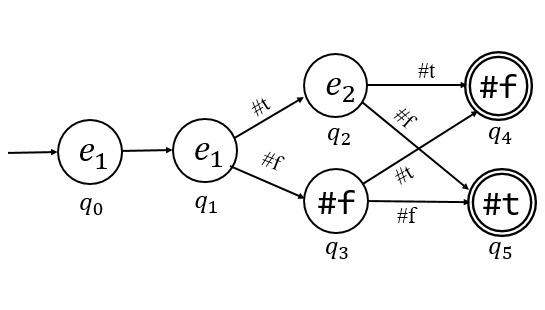
\includegraphics[scale=0.28]{images/ifa/ifa-nand-4.png}
        }
        \subcaptionbox{After Simplification\label{fig:ifa-nand-as}}[.45\linewidth]{
            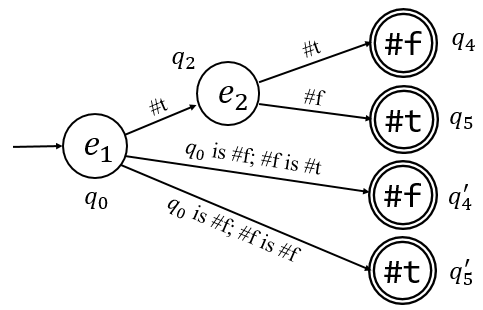
\includegraphics[scale=0.28]{images/ifa/ifa-nand.png}
        }
        \caption{IFA of \m{nand}}
        \label{fig:ifa-nand-std}
    \end{figure}

    Start with $q_0$, we get a context rule as
    \[
        \infer{(\m{nand}~e_1~e_2) \to (\m{nand}~e_1'~e_2)}{e_1 \to e_1'}
    \]
    % \infrule[E-Nand]{e_1 \to e_1'}{(\m{nand}~e_1~e_2) \to (\m{nand}~e_1'~e_2)}

    We first discuss the branch of $q_2$. Add $e_1~\key{is}~\m{\#t}$ to $T$. Because $q_2$ is not a terminal node, add a new context rule for $q_2$.
    \[
        \infer{(\m{nand}~e_1~e_2) \to (\m{nand}~e_1~e_2')}{e_2 \to e_2'\quad e_1~\key{is}~\m{\#t}}
    \]
    % \infrule[E-NandTrue]{e_2 \to e_2'\quad e_1~\key{is}~\m{\#t}}{(\m{nand}~e_1~e_2) \to (\m{nand}~e_1~e_2')}

    Since $q_4$ is a reduction rule, append $e_2~\key{is}~\m{\#t}$ to $T$ and add a new reduction rule for $q_4$. Reduction rule for $q_5$ is similar.
    \[
        \begin{array}{c}
            \infer{(\m{nand}~e_1~e_2) \to \m{\#f}}{e_1~\key{is}~\m{\#t}\quad e_2~\key{is}~\m{\#t}}
            \quad
            \infer{(\m{nand}~e_1~e_2) \to \m{\#t}}{e_1~\key{is}~\m{\#t}\quad e_2~\key{is}~\m{\#f}}
        \end{array}
    \]
    % \infrule[E-NandTrueTrue]{e_1~\key{is}~\m{\#t}\quad e_2~\key{is}~\m{\#t}}{(\m{nand}~e_1~e_2) \to \m{\#f}}
    % \infrule[E-NandTrueFalse]{e_1~\key{is}~\m{\#t}\quad e_2~\key{is}~\m{\#f}}{(\m{nand}~e_1~e_2) \to \m{\#t}}

    Back to $q_0$, for $q_4'$ and $q_5'$ are also terminal nodes, we can build reduction rules for $q_4'$ and $q_5'$ in the same way.
    \[
        \begin{array}{c}
            \infer{(\m{nand}~e_1~e_2) \to \m{\#f}}{e_1~\key{is}~\m{\#f}\quad \m{\#f}~\key{is}~\m{\#t}}
            \quad
            \infer{(\m{nand}~e_1~e_2) \to \m{\#t}}{e_1~\key{is}~\m{\#f}\quad \m{\#f}~\key{is}~\m{\#f}}
        \end{array}
    \]
    % \infrule[E-NandFalse1]{e_1~\key{is}~\m{\#f}\quad \m{\#f}~\key{is}~\m{\#t}}{(\m{nand}~e_1~e_2) \to \m{\#f}}
    % \infrule[E-NandFalse2]{e_1~\key{is}~\m{\#f}\quad \m{\#f}~\key{is}~\m{\#f}}{(\m{nand}~e_1~e_2) \to \m{\#t}}

    We can judge that \m{\#f} is not \m{\#t}, so we can remove the rule (NandFalse1) from the rules, for it contains a condition that is never met. At the same time, we rewrite the remaining rules into a more customary form.
    \[
        \begin{array}{cc}
            \infer{(\m{nand}~e_1~e_2) \to (\m{nand}~e_1'~e_2)}{e_1 \to e_1'}
             &
            \infer{(\m{nand}~\m{\#t}~e_2) \to (\m{nand}~\m{\#t}~e_2')}{e_2 \to e_2'}
        \end{array}
    \]\[
        \begin{array}{ccc}
            (\m{nand}~\m{\#t}~\m{\#t}) \to \m{\#f}
             &
            (\m{nand}~\m{\#t}~\m{\#f}) \to \m{\#t}
             &
            (\m{nand}~\m{\#f}~e_2) \to \m{\#t}
        \end{array}
    \]
    \myend
\end{example}
% \infrule[E-Nand]{e_1 \to e_1'}{(\m{nand}~e_1~e_2) \to (\m{nand}~e_1'~e_2)}
% \infrule[E-NandTrue]{e_2 \to e_2'}{(\m{nand}~\m{\#t}~e_2) \to (\m{nand}~\m{\#t}~e_2')}
% \infax[E-NandTrueTrue]{(\m{nand}~\m{\#t}~\m{\#t}) \to \m{\#f}}
% \infax[E-NandTrueFalse]{(\m{nand}~\m{\#t}~\m{\#f}) \to \m{\#t}}
% \infax[E-NandFalse]{(\m{nand}~\m{\#f}~e_2) \to \m{\#t}}


%--------------------------
\subsubsection{Correctness}

\begin{lemma}
    \label{lemma:ifa2rule-correct}
    For any language construct \m{H}, if its normal IFA meets the above assumptions, the evaluation rules obtained according to the algorithm in Theorem \ref{mythm:ifa2rule} have the same semantics as IFA.
\end{lemma}

%In other words, for any term of language construct \m{H}, evaluating the term by IFA and evaluating by rule get the same derivation sequence.

\begin{proof}
    %[Proof of Lemma \ref{lemma:ifa2rule-correct}]
    We only need to discuss that in a one-step derivation, both get the same result.

    Considering an expression $e=(\m{H}~e_1 \ldots e_n)$ use rule $r$ to derive. The expression $e$ must meet the condition $T$ of $r$ such as some parameters must be value or a specific value. Suppose $r$ is generated by node $q$. Then $T$ is the set of all transition conditions from $q_0$ to $q$. Therefore, the one-step derivation of this expression $e$ in IFA must be located at $q$. If $r$ is a context rule for a pattern variable $e_i$, the expression of $q$ is $e_i$ as well, and $e_i$ of $e$ is not a value. Thus both of the one-step derivation of $e$ are one-step derivation of $e_i$.

    Similarly, if an expression can be derived in one step in IFA, then it must be able to use the corresponding rule for one-step derivation.
\end{proof}

%===========================
\subsection{Deriving Evaluation Rules for Syntactic Sugars}

As we have seen in Example \ref{ex:nand}, although  the rules of \m{nand} contain the use of the language construct of \m{if}, the final derived IFA does not. We can apply this procedure to derive reductions rules for each syntactic sugar: construct an  IFA for the  syntactic sugar, simplify it and convert it into rules.
%With the IFA, we can easily get the evaluation rules for syntactic sugars.

Similarly, we also need to add some constraints on syntactic sugar.

\begin{Asm}[Orderliness of Syntactic Sugar]
    \label{Asm:orderliness-sugar}
    The definition of each syntactic sugar can only use the language construct in core language and the syntactic sugar that has been defined.
\end{Asm}

\begin{Def}
    \label{def:ifa-sugar}
    Considering the following syntactic sugar
    \[
        \drule{(\m{SurfHead}~x_1~\ldots~x_n)}{e},
    \]
    the IFA of \m{SurfHead} is defined as the IFA of language construct \m{SurfHead'} whose evaluation rule is
    \[
        (\m{SurfHead'}~x_1~\ldots~x_n) \to e
    \]

\end{Def}

%--------------------------------------------
\begin{example}

    Suppose that there are only \m{if} and \m{let} in our core language, whose IFAs are known. Now we build rules for syntactic sugar \m{Or}.
    \[
        \drule{(\m{Or}~e_1~e_2)}{(\m{let}~x~e_1~(\m{if}~x~x~e_2))}
    \]

    \begin{figure}[t]
        \centering
        \subcaptionbox{Rule of Definition \ref{def:ifa-sugar} \label{fig:ifa-ex-or-1}}[.31\linewidth]{
            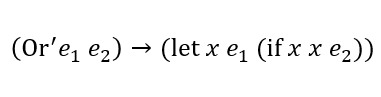
\includegraphics[scale=0.3]{images/ifa/ifa-ex-or-1.png}
        }
        \subcaptionbox{IFA generated with the algorithm of Theorem \ref{mythm:Rule2IFA} \label{fig:ifa-ex-or-2}}[.31\linewidth]{
            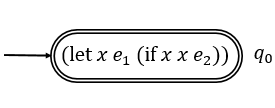
\includegraphics[scale=0.3]{images/ifa/ifa-ex-or-2.png}
        }
        \subcaptionbox{Expand language construct of \m{let} \label{fig:ifa-ex-or-3}}[.31\linewidth]{
            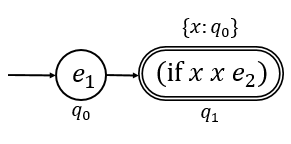
\includegraphics[scale=0.3]{images/ifa/ifa-ex-or-3.png}
        }
        \subcaptionbox{Expand language construct of \m{if} \label{fig:ifa-ex-or-4}}[.31\linewidth]{
            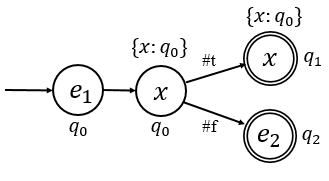
\includegraphics[scale=0.3]{images/ifa/ifa-ex-or-4.png}
        }
        \subcaptionbox{Replace $x$ with expression according to the symbol table \label{fig:ifa-ex-or-5}}[.31\linewidth]{
            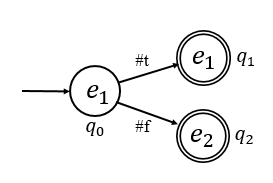
\includegraphics[scale=0.3]{images/ifa/ifa-ex-or-5.png}
        }
        \subcaptionbox{Rules generated with the algorithm of Theorem \ref{mythm:ifa2rule} \label{fig:ifa-ex-or-6}}[.31\linewidth]{
            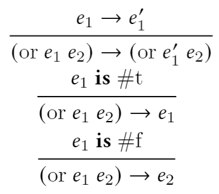
\includegraphics[scale=0.3]{images/ifa/ifa-ex-or-6.png}
        }
        \caption{Example: Syntactic Sugar of \m{or}}
        \label{fig:ifa-nand-std}
    \end{figure}

    The \m{Or} syntactic sugar only uses the syntax structure of the core language, which meets Assumption \ref{Asm:orderliness-sugar}, so we can generate evaluation rules for \m{Or}.
    %
    The IFA of \m{Or} is the same as the IFA of \m{Or'} whose rule is shown in Figure \ref{fig:ifa-ex-or-1}. Therefore, we can generate an IFA according to the rule as shown in Figure \ref{fig:ifa-ex-or-2}. Next we transform IFA to make it a normal IFA, as shown in Figure \ref{fig:ifa-ex-or-3} to Figure \ref{fig:ifa-ex-or-5}. Finally, according to the structure of IFA, generate or evaluation rules, as shown in Figure \ref{fig:ifa-ex-or-6}.
    \myend
\end{example}

% \infrule[E-Or]{e_1 \to e_1'}{(\m{Or}~e_1~e_2) \to (\m{Or}~e_1'~e_2)}
% \infrule[E-OrTrue]{e_1~\key{is}~\m{\#t}}{(\m{Or}~e_1~e_2) \to e_1}
% \infrule[E-OrFalse]{e_1~\key{is}~\m{\#f}}{(\m{Or}~e_1~e_2) \to e_2}

%--------------------------
%\subsubsection{Correctness}

As discussed in Section \ref{sec3}, our approach should satisfy the three properties: emulation, abstraction and coverage. The property of abstraction is obvious, for the rules we generate only contain the language construct itself, without any other structures in core language. However, our approach does not perfectly satisfy emulation and coverage. In the derivation, we lost the information that a language construct is reduced to another language construct. This makes the derivation sequence different. But through Theorem \ref{mythm:nmlifa}, Lemma \ref{lemma:rule2ifa-correct} and Lemma \ref{lemma:ifa2rule-correct}, we can guarantee the correctness of the evaluation results.

Another issue is the expressiveness of IFA. As discussed above, we can well support general syntactic sugar and hygieneinderive sugar. But we require that when constructing IFA, the IFA of all its substructures is known. So at present we have difficulty dealing with recursive sugar. In addition, when we construct rules from IFA, if the deformation of IFA causes it to not satisfy the assumption \ref{Asm:st}, the rules cannot be generated. This would not happen in a core language with only \m{if} and \m{let}. But for a more complex language, this situation may exist.
%!TEX root = ./main.tex
\section{Implementation and Case Studies}
\label{sec5}


\subsection{Implementation}

Our resugaring approach is implemented using PLT Redex\cite{SEwPR}, which is a semantic engineering tool based on reduction semantics\cite{reduction}. The framework of the implementation is as Figure \ref{fig:frame}.
In the language model, desugaring rules are written as reduction rules of \m{SurfExp}. And context rules of \m{SurfExp} have no restriction (every subexpression is reducible as a hole). Then for each resugaring step, we should choose the exact reduction which satisfies the reduction of mixed language's reduction rule  in Section \ref{mark:mixedreduction}.
\begin{figure}[t]
	\centering
	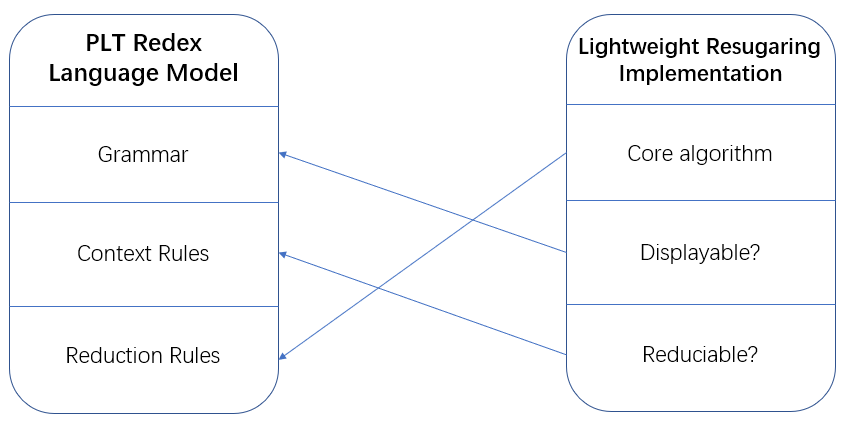
\includegraphics[width=5cm]{images/frame.png}
	\caption{Framework of Implementation}
	\label{fig:frame}
\end{figure}



\ignore{
\label{mark:blackbox}
And one may notice the traditional resugaring approach does not need the whole evaluation rules of core language, a black-box stepper is enough instead. Our approach can also work by  given a black-box stepper with a tricky extension, but a little more information is needed. Here we introduce the extension firstly.
We use $\redc{}{}$ to denote a reduction step of core language's expression in the black-box stepper, and $\rede{}{}$ to denote a step in the extension evaluator for the mixed language. We may use $\redm{}{}$ to denote the one-step reduction in our mixed language, defined in Section \ref{mark:mixedreduction}.
\infrule[CoreRed]
{ \forall~i.~e_i\in \m{CoreExp}\\
\redc{(\m{CoreHead}~e_1~\ldots~e_n)}{e'}}
{\rede{(\m{CoreHead}~e_1~\ldots~e_n)}{e'}}
\infrule[CoreExt1]
{ \forall~i.~tmp_i= (e_i \in \m{SurfExp}~?~\m{tmpe}~:~e_i),~where~\m{tmpe}~is~any~reduciable~\m{CoreExp}~term\\
\redc{(\m{CoreHead}~tmp_1~\ldots~tmp_i~\ldots~tmp_n)}{(\m{CoreHead}~tmp_1~\ldots~tmp_i'~\ldots~tmp_n)}}
{\rede{(\m{CoreHead}~e_1~\ldots~e_i~\ldots~e_n)}{(\m{CoreHead}~e_1~\ldots~e_i'~\ldots~e_n)}\\where~\redm{e_i}{e_i'}~if~e_i~\in~\m{SurfExp},~else~\rede{e_i}{e_i'}}
\infrule[CoreExt2]
{ \forall~i.~tmp_i= (e_i \in \m{SurfExp}~?~\m{tmpe}~:~e_i),~where~\m{tmpe}~is~any~reduciable~\m{CoreExp}~term\\
\redc{(\m{CoreHead}~tmp_1~\ldots~tmp_n)}{e'}~\note{// not reduced in subexpressions}}
{\rede{(\m{CoreHead}~e_1~\ldots~e_n)}{e'[e_1/tmp_1~\ldots~e_n/tmp_n]}}
Then we should replace the rules \m{CoreRed1} and \m{CoreRed2} by the following rule.
\infrule[ExtRed]
{\rede{(\m{CoreHead}~e_1~\ldots~e_n)}{e'}}
{\redm{(\m{CoreHead}~e_1~\ldots~e_n)}{e'}}

Putting them in simple words. For expression \Code{(CoreHead $e_1$ $\ldots$ $e_n$)} whose subexpressions contain \m{SurfExp}, replacing all \m{SurfExp} subexpressions not in core language with any reducible core language's term \m{tmpe}. Then getting a result after inputting the new expression $e'$ to the original black-box stepper. If reduction appears at a subexpression at $e_i$ or what the $e_i$ replaced by, then the stepper with the extension should return \Code{(CoreHead $e_1$ $\ldots$ $e_i'$ $\ldots$ $e_n$)}, where $e_i'$ is $e_i$ after the mixed language's one-step reduction ($\redm{}{}$) or after core language's reduction with extension ($\rede{}{}$) (rule \m{CoreExt1}, an example in Figure \ref{fig:e1}). Otherwise, the stepper should return \Code{$e'$}, with all the replaced subexpressions replacing back (rule \m{CoreExt2}, an example in Figure \ref{fig:e2}). The extension will not violate the properties of original core language's evaluator. It is obvious that the evaluator with the extension will reduce at the subexpression as it needs in core language, if the reduction appears in a subexpression. One may notice that the stepper with extension behaves the same as mixing the evaluation rules of core language and desugaring rules of surface language. The extension is just to make it works when the evaluator of core language is a black-box stepper, by getting context rules using the \m{tmpe}. That's why the extension is tricky.
\reduce{can be simplified}

\begin{center}
\begin{figure}[thb]
\centering
\Code{(if (and e1 e2) true false)}\\ $\Downarrow_{replace}$\\ \Code{(if tmpe1 true false)}\\ $\Downarrow_{blackbox}$\\ \Code{(if tmpe1' true false)}\\ $\Downarrow_{desugar}$\\ \Code{(if (if e1 e2 false) true false)}
\caption{\m{CoreExt1}'s Example}
\label{fig:e1}
\end{figure}

\begin{figure}[thb]
\centering
\Code{(if (if true ture false) (and ...) (or ...))}\\ $\Downarrow_{replace}$ \\\Code{ (if (if true ture false) tmpe2 tmpe3)}\\ $\Downarrow_{blackbox}$\\  \Code{(if true tmpe2 tmpe3)}\\ $\Downarrow_{replaceback}$\\ \Code{(if true (and ...) (or ...))}
\caption{\m{CoreExt2}'s Example}
\label{fig:e2}
\end{figure}


\end{center}

But something goes wrong when substitution takes place during \m{CoreExt2}. Just as the example we will talk about later in Section \ref{mark:hygienic}, for a expression like \Code{(let x 2 (Sugar x 1))}, it should reduce to \Code{(Sugar 2 1)} by the \m{CoreRed2} rule, but got \Code{(Sugar x 1)} by the \m{CoreExt2} rule. So when using the extension of black-box stepper's rule (\m{ExtRed2}), we need some other information about in which subexpression a substitution will take place (the substitution can be got by a similar idea as the tricky extension). Then for these subexpressions, we need to do the same substitution before replacing back.
}
% \todo{black-box's extension was removed, maybe add in appendix}



\label{mark:optimize}
Note that in \m{SurfRed1} rule and \m{CoreExt1} rule, there is a recursive call on $\redm{}{}$. We can optimize the resugaring algorithm by recursively resugaring. For example, \Code{(Sugar1 (Sugar2  ...) ...)} as the input, and find the first subexpression should be reduced. We can first get the resugaring sequences of \Code{(Sugar2 ...)} as Figure \ref{fig:subsequence}, then the resugaring sequences is got as \ref{fig:optimized}. Thus, we will not need to try to expand the outermost sugar for each inner step (recursively resugaring for inner expression).

\begin{figure}[t]
\centering
\subcaptionbox{Subsequences of \m{Sugar2} \label{fig:subsequence}}[.45\linewidth]{
\begin{flushleft}
{\small
\begin{Codes}
\qquad (Sugar2 ...)\\
  \OneStep{ exp1}\\
\DeStep{\quad expi} \note{//0 or more steps}\\
\OneStep{ expn}
\end{Codes}
}
\end{flushleft}
}
\subcaptionbox{Optimized Resugaring of \m{Sugar1} \label{fig:optimized}}[.45\linewidth]{
\begin{flushleft}
{\small
\begin{Codes}
\qquad (Sugar1 (Sugar2 ...) ...)\\
  \OneStep{ (Sugar1 exp1 ...)}\\
\DeStep{\quad(Sugar1 expi ...)} \note{//0 or more steps}\\
\OneStep{ (Sugar1 expn ...)}
\end{Codes}
}
\end{flushleft}
}
\caption{Recursive Optimization's Example}
\label{fig:optimize}
\end{figure}


As for the automatic derivation of evaluation rules, we implement a simple demo by writing some core language's IFAs (such as \m{if}, \m{let}) manually, because it is enough to do some case studies for the resugaring tasks.

\subsection{Case Studies}



We test some applications on the tool as case studies. Some examples we will discuss in this section are in Figure \ref{fig:resugaring}. Note that we set call-by-value lambda calculus as terms in \m{CommonExp}, because we need to output some intermediate sequences including lambda expressions in some examples. It's easy if we want to skip them. \todo{modify drule or simplify Codes}

\begin{figure}[t]
\centering
\subcaptionbox{Example of SKI\label{fig:SKI}}[.3\linewidth]{
\begin{flushleft}
{\scriptsize
\begin{Codes}
\qquad (S (K (S I)) K xx yy)\\
\OneStep{ (((K (S I)) xx (K xx)) yy)}\\
\OneStep{ (((S I) (K xx)) yy)}\\
\OneStep{ (I yy ((K xx) yy))}\\
\OneStep{ (yy ((K xx) yy))}\\
\OneStep{ (yy xx)}

\end{Codes}
}
\end{flushleft}
}
\subcaptionbox{Example of \m{Hygienicadd}\label{fig:hygienicadd}}[.32\linewidth]{
\begin{flushleft}
{\scriptsize
\begin{Codes}
\qquad    (let x 2 (Hygienicadd 1 x))\\
\OneStep{ (Hygienicadd 1 2)}\\
\OneStep{ (+ 1 2)}\\
\OneStep{ 3}\\

\end{Codes}

}
\end{flushleft}
}
\subcaptionbox{Example of \m{Let}\label{fig:Let}}[.36\linewidth]{
\begin{flushleft}
{\scriptsize
\begin{Codes}
\qquad    (Let x 1 (+ x (Let x 2 (+ x 1))))\\
\OneStep{ (Let x 1 (+ x (+ 2 1)))}\\
\OneStep{ (Let x 1 (+ x 3))}\\
\OneStep{ (+ 1 3)}\\
\OneStep{ 4}\\
\end{Codes}
}
\end{flushleft}
}

%newline
\subcaptionbox{Example of \m{Odd} and \m{Even}\label{fig:oddeven}}[.3\linewidth]{
\begin{flushleft}
{\scriptsize
\begin{Codes}
\qquad    (Odd 2)\\
\OneStep{ (Even (- 2 1))}\\
\OneStep{ (Even 1)}\\
\OneStep{ (Odd (- 1 1))}\\
\OneStep{ (Odd 0)}\\
\OneStep{ \#f}
\end{Codes}
}
\end{flushleft}
}
\subcaptionbox{Example of \m{Map}\label{fig:Map}}[.55\linewidth]{
\begin{flushleft}
{\scriptsize
\begin{Codes}
    \qquad(Map (lambda (x) (+ x 1)) (cons 1 (list 2)))\\
\OneStep{ (Map (lambda (x) (+ x 1)) (list 1 2))}\\
\OneStep{ (cons 2 (Map (lambda (x) (+ 1 x)) (list 2)))}\\
\OneStep{ (cons 2 (cons 3 (Map (lambda (x) (+ 1 x)) (list))))}\\
\OneStep{ (cons 2 (cons 3 (list)))}\\
\OneStep{ (cons 2 (list 3))}\\
\OneStep{ (list 2 3)}
\end{Codes}
}
\end{flushleft}
}
\subcaptionbox{Example of \m{Filter}\label{fig:Filter}}[.9\linewidth]{
\begin{flushleft}
{\scriptsize
\begin{Codes}
    \qquad(Filter (lambda (x) (and (> x 1) (< x 4))) (list 1 2 3 4))\\
\OneStep{ (Filter (lambda (x) (and (> x 1) (< x 4))) (list 2 3 4))}\\
\OneStep{ (cons 2 (Filter (lambda (x) (and (> x 1) (< x 4))) (list 3 4)))}\\
\OneStep{ (cons 2 (cons 3 (Filter (lambda (x) (and (> x 1) (< x 4))) (list 4))))}\\
\OneStep{ (cons 2 (cons 3 (Filter (lambda (x) (and (> x 1) (< x 4))) (list))))}\\
\OneStep{ (cons 2 (cons 3 (list)))}\\
\OneStep{ (cons 2 (list 3))}\\
\OneStep{ (list 2 3)}
\end{Codes}

}
\end{flushleft}
}
\caption{Resugaring Examples}
\label{fig:resugaring}
\end{figure}


\subsubsection{Simple sugar}
\label{mark:simple}

We construct some simple syntactic sugars and try it on our tool. Some sugar is inspired by the first work of resugaring\cite{resugaring}. The result shows that our approach can handle all sugar features of their first work.
Take an SKI combinator syntactic sugar as an example.
\[
\begin{array}{l}
\drule{\m{S}}{\Code{(lambdaN (x1 x2 x3) (x1 x2 (x1 x3)))}}\\
\drule{\m{K}}{\Code{(lambdaN (x1 x2) x1)}}\\
\drule{\m{I}}{\Code{(lambdaN (x) x)}}
\end{array}
\]




Although SKI combinator calculus is a reduced version of lambda calculus, we can construct combinators' sugar based on call-by-need lambda calculus in our core language. For sugar expression \Code{(S (K (S I)) K xx yy)}, we get the resugaring sequences as Figure \ref{fig:SKI}. During the test, we find 33 intermediate steps are needed after the totally desugaring of the input expression, but only 5 of them can be returned to the surface, so many attempts to reverse the desugaring would fail if using the traditional resugaring approach, in such a little expression. That's why lazy desugaring makes our approach efficient.




\ignore{
  For the traditional approach, the sugar expression should firstly desugar to
\begin{Codes}
((lambdaN (x1 x2 x3) (x1 x3 (x2 x3)))
  ((lambdaN (x1 x2) x1)
   ((lambdaN  (x1 x2 x3) (x1 x3 (x2 x3)))
    (lambdaN (x) x)))
  (lambdaN (x1 x2) x1)
  xx yy)
\end{Codes}
\reduce{can be removed}

Then in our core language, the execution of expanded expression will contain 33 reduction steps in our implementation. For each step, there will be many attempts to match and substitute the syntactic sugars to resugar the expression. It will omit more steps for a larger expression.
}

As for the derivation of syntactic sugar's evaluation rules, we have shown an example of \m{and} sugar and \m{or} sugar in overview. But what if the \m{or} sugar written as follows?
\[\drule{\Code{(or $e_1$ $e_2$)}}{\Code{(let x $e_1$ (if x x $e_2$))}}\]
Of course, we got the same evaluation rules as the example in overview.
\[
\begin{array}{c}
\infer {(\mbox{or}~e_1~e_2) \rightarrow (\mbox{or}~e_1'~e_2)} {e_1~ \rightarrow~e_1'}
\qquad
(\mbox{or}~\#t~e2) \rightarrow \#t
\quad
(\mbox{or}~\#f~e2) \rightarrow e_2 \\
\end{array}
\]

Then for expressions headed with \m{or}, we won't need the one-step try to figure out whether desugaring or processing on a subexpression, which makes our approach more concise. Overall, the unidirectional resugaring algorithm makes our approach efficient, because no attempts for resugaring the expression are needed.
\subsubsection{Hygienic sugar}
\label{mark:hygienic}


The second work\cite{hygienic} of traditional resugaring approach mainly processes hygienic sugar compared to first work. It uses a DAG to represent the expression. However, hygiene is not hard to be handled by our lazy desugaring strategy. Our algorithm can easily process hygienic sugar without a special data structure.
A typical hygienic problem is as the following example.
\[
\drule{\Code{(Hygienicadd $e_1$ $e_2$)}}{\Code{(let x $e_1$ (+ x $e_2$))}}
\]
% \begin{Codes}
% 	(Hygienicadd e1 e2) \DeStep{ (let ((x e1)) (+ x e2))}
% \end{Codes}
For traditional resugaring approach, if we want to get sequences of \Code{(let x 2 (Hygienicadd 1 x))}, it will firstly desugar to \Code{(let x 2 (let x 1 (+ x x)))}, which is awful because the two $x$ in \Code{(+ x x)} should be bind to different value. So the traditional hygienic resugaring approach uses abstract syntax DAG to distinct different \m{x} in the desugared expression. But for our approach based on lazy desugaring, the \m{hygienicadd} sugar does not have to desugar until necessary, thus, getting resugaring sequences as Figure \ref{fig:hygienicadd} based on a rewriting system which renaming the variables during the rewriting. \todo{@zc: different values?; what's  meaning of the sentence after "thus"}


The lazy desugaring is also convenient for hygienic resugaring for non-hygienic rewriting. For example, \Code{(let x 1 (+ x (let x 2 (+ x 1))))} may be reduced to \Code{(+ 1 (let 1 2 (+ 1 1)))} by a simple core language whose \Code{let} expression does not handle cases like that. But by writing a simple sugar Let,
\[\drule{\Code{(Let~$e_1$~$e_2$~$e_3$)}}{\Code{(let~($e_1$~$e_2$)~$e_3$)}}\]
and making some simple modifies in the reduction of mixed language, we will get the resugaring sequences as Figure \ref{fig:Let} in our tool. todo{@zc: let (e e) e -> let e e e; support Let now?}


In practical application, we think hygiene can be easily processed by rewriting systems, so we just use a rewriting system which can rename variable automatically.

And for the derivation method, there is no rewriting system at all, but the hygiene is handled more concisely. we build a hygienic sugar \m{Hygienicor} based on the \m{or} sugar.
\[
\begin{array}{l}
\drule{\Code{(Or $e_1$ $e_2$)}}{\Code{(let x $e_1$ (if x x $e_2$))}}\\
\drule{\Code{(Hygienicor $e_1$ $e_2$)}}{\Code{(let x $e_1$ (or $e_2$ x))}}
\end{array}
\]
Though no need to write the sugar like that, something wrong may happen without hygienic rewriting system (\Code{(if x x x)} appears). But with the step in normalization of IFA introduced in \ref{mark:hygieneinderive}, we can easily get the following rules, which will behave as it should be in resugaring. \todo{@zc: Because we have replaced x with expression when constructing normal IFA of or, the binding of x will not cause conflicts.}
\[
\begin{array}{c}
\infer {(\mbox{Hygienicor}~e_1~e_2) \rightarrow (\mbox{Hygienicor}~e_1'~e_2)} {e_1~ \rightarrow~e_1'}
\qquad
\infer {(\mbox{Hygienicor}~v_1~e_2) \rightarrow (\mbox{Hygienicor}~v_1~e_2')} {e_2~ \rightarrow~e_2'}
\end{array}\]
\[
\begin{array}{c}
(\mbox{Hygienicor}~v_1~\#t) \rightarrow \#t
\quad
(\mbox{Hygienicor}~v_1~\#f) \rightarrow v_1
\end{array}
\]

Overall, our result shows lazy desugaring is really a good way to handle hygienic sugar in any systems.

\subsubsection{Recursive sugar}
\label{sec:recursiveSugar}

Recursive sugar is a kind of syntactic sugars where call itself or each other during the expanding. For example,
\[
\begin{array}{l}
\drule{(\m{Odd}~$e$)~}{\Code{(if (> $e$ 0) (Even (- $e$ 1)) \false)}}\\
\drule{(\m{Even}~$e$)}{\Code{(if (> $e$ 0) (Odd (- $e$ 1)) \true)}}
\end{array}
\]
are common recursive sugars. The traditional resugaring approach can't process syntactic sugar written like this (non-pattern-based) easily, because boundary conditions are in the sugar itself.

Take \Code{(Odd 2)} as an example. The previous work will firstly desugar the expression using the rewriting system. Then the rewriting system will never terminate as following shows.
\begin{scriptsize}
\begin{Codes}
   (Odd 2)
\DeStep{ (if (> 2 0) (Even (- 2 1) \#f))}
\DeStep{ (if (> (- 2 1) 0) (Odd (- (- 2 1) 1) \#t))}
\DeStep{ (if (> (- (- 2 1) 1) 0) (Even (- (- (- 2 1) 1) 1) \#f))}
\DeStep{ ...}
\end{Codes}
\end{scriptsize}



Then the advantage of our approach is embodied. Our lightweight approach doesn't require a whole expanding of sugar expression, which gives the framework chances to judge boundary conditions in sugars themselves, and showing more intermediate sequences. We get the resugaring sequences as Figure \ref{fig:oddeven} of the former example using our tool.



We also construct some higher-order syntactic sugars and test them. The higher-order feature is important for constructing practical syntactic sugars. And many higher-order sugars should be constructed by recursive definition. The first sugar is \m{Filter}, implemented by pattern matching term rewriting.
\[\begin{array}{l}
\drule{\Code{(Filter $e$ (list $v_1$ $v_2$ ...))}}{}\\
\qquad\Code{(if ($e$ $v_1$) (cons $v_1$ (Filter $e$ (list $v_2$ ...)))\ (Filter $e$ (list $v_2$ ...)))}\\
\drule{\Code{(Filter $e$ (list))}}{\Code{(list)}}
\end{array}\]
and getting resugaring sequences as Figure \ref{fig:Filter}.
Here, although the sugar can be processed by traditional resugaring approach, it will be redundant. The reason is that, a Filter for a list of length $n$ will match to find possible resugaring $n*(n-1)/2$ times. Thus, lazy desugaring is really important to reduce the resugaring complexity of recursive sugar.

Moreover, just like the \emph{Odd and Even} sugar above, there are some simple rewriting systems which do not allow pattern-based rewriting. Or there are some sugars that need to be expressed by the terms in core language as rewriting conditions. Take the example of another higher-order sugar \m{Map} as an example, and get resugaring sequences as Figure \ref{fig:Map}.
\[
\begin{array}{l}
\drule{\Code{(Map $e_1$ $e_2$)}}{}\\
\Code{(let x $e_2$ (if (empty? x) (list) (cons ($e_1$ (first x)) (Map $e_1$ (rest x)))))}
\end{array}
\]



Note that the \m{let} term is to limit the subexpression only appears once in RHS. In this example, we can find that the list \Code{(cons 1 (list 2))}, though equal to \Code{(list 1 2)}, is represented by core language's term. So it will be difficult to handle such inline boundary conditions for traditional rewriting systems. But our approach is easy to handle cases like this. So our resugaring approach by lazy desugaring is powerful.

\todo{@zc: whether it is necessary to discuss ifa cannot do this}

%!TEX root = ./main.tex
\section{Related Work}
\label{sec6}
%Explain the work that are related to your problem, and to your three contributions.
\todo{checking the sentense}

As discussed many times before, our work is much related to the pioneering work of \emph{resugaring} in \cite{resugaring}. The idea of "tagging" and "reverse desugaring" is a clear explanation of "resugaring", but it becomes very complex when the RHS of the desugaring rule becomes complex. Our approach does not need to reverse desugaring and is more powerful, and efficient.
For hygienic resugaring, compared with the approach of using DAG to solve the variable binding problem in \cite{hygienic}, our approach of "lazy desugaring" can achieve a kind of natural hygiene within our core language.



\emph{Macros as multi-stage computations} \cite{multistage} is a work related to our lazy expansion for sugars. Some other researches \cite{modularstaging} about multi-stage programming \cite{MSP} indicate that it is useful for implementing domain-specific languages. However, multi-stage programming is a metaprogramming method, which mainly works for run-time code generation and optimization. In contrast, our lazy resugaring approach treats sugars as part of a mixed language, rather than separate them by staging. Moreover, the lazy desugaring gives us a chance to derive evaluation rules of sugars, which is a new good point compared to multi-stage programming.

Our work is related to the \emph{Galois slicing for imperative functional programs} \cite{slicing}, a work for dynamic analyzing functional programs during execution. The forward component of the Galois connection maps a partial input $x$ to the greatest partial output $y$ that can be computed from $x$; the backward component of the Galois connection maps a partial output $y$ to the least partial input $x$ from which we can compute $y$.
%Our approach used a similar idea on slicing expressions and processing on subexpressions.
This can also be considered as a bidirectional transformation \cite{bx,lens07} and the round-tripping between desugaring and resugaring in the existing approach. In contrast to these works, our resugaring approach is basically unidirectional. 


There is a long history of hygienic macro expansion\cite{hygienicmacro}, and a formal specific hygiene definition was given \cite{10.5555/1792878.1792884} by specific the binding scopes of macros. another formal definition of the hygienic macro\cite{EssenceofHygiene} is based on nominal logic\cite{10.1007/s001650200016}. Instead of using the desugaring rule or something else to achieve hygiene, we use the lazy desugaring with the small core language to avoid hygienic problems in our approach.
%
%When the tracking in their notation can be easily done for sugar whose rules can be derived automatically.

Our implementation is built upon the PLT Redex \cite{SEwPR}, a semantics engineering tool, but it is possible to implement our approach on other semantics engineering tools such as those in \cite{dynsem,Ksemantic} which aim to test or verify the semantics of languages. The methods of these researches can be easily combined with our approach to implementing more general rule derivation. \emph{Ziggurat} \cite{Ziggurat} is a semantic extension framework, also allowing defining new macros with semantics based on existing terms in a language. It is should be useful for static analysis of macros.
%Instead of semantics based on core language, the reduction rules of sugar derived by our approach are independent of the core language, which may be more concise for static analysis.


%!TEX root = ./main.tex
\section{Conclusion}
\label{sec7}

%Summarize the paper, explaining what you have shown, what results you have achieved, and what future work is.

In this paper, we propose a novel resugaring approach using lazy desugaring. We design the approach based on a  core language, with a simple desugaring system. Our algorithm then can output the evaluation sequence in the surface syntax, given some syntactic sugars together with an input program. In our approach, the most important insight is delaying the expansion of syntactic sugars by calculating context rules (Section \ref{sec:language} and \ref{sec:algo}), which decide whether the mixed language should reduce the sub-expression by core's reduction rules or expand the sugar. We show that the system can handle a variety of syntactic sugars and can achieve better efficiency (Section \ref{mark:resugaringexample} and \ref{sec:implementation}). Moreover, the approach is flexible to make some extensions (Section \ref{sec:ext}).

We find the extensions may work if the core language and the syntactic sugar have some properties such like compositional, clear semantics, and unique computational order. So one possible future work of this is to extend the core language and the desugaring system with other components of language design like type system, analyzer, and optimizer. Also, we find it is possible to derive stand-alone evaluation rules for the surface language by means similar to how we calculate context rules, making it more convenient to develop domain-specific languages. This functionality can be added to future systems.


%% Acknowledgments
\begin{acks}                            %% acks environment is optional
                                        %% contents suppressed with 'anonymous'
  %% Commands \grantsponsor{<sponsorID>}{<name>}{<url>} and
  %% \grantnum[<url>]{<sponsorID>}{<number>} should be used to
  %% acknowledge financial support and will be used by metadata
  %% extraction tools.
  This material is based upon work supported by the
  \grantsponsor{GS100000001}{National Science
    Foundation}{http://dx.doi.org/10.13039/100000001} under Grant
  No.~\grantnum{GS100000001}{nnnnnnn} and Grant
  No.~\grantnum{GS100000001}{mmmmmmm}.  Any opinions, findings, and
  conclusions or recommendations expressed in this material are those
  of the author and do not necessarily reflect the views of the
  National Science Foundation.
\end{acks}


%% Bibliography
\bibliography{reference}


%% Appendix
\appendix
\section{Appendix}

Text of appendix \ldots

\end{document}
